%------------------------------------------------------------------------------
% Beginning of journal.tex
%------------------------------------------------------------------------------
%
% AMS-LaTeX version 2 sample file for journals, based on amsart.cls.
%
%        ***     DO NOT USE THIS FILE AS A STARTER.      ***
%        ***  USE THE JOURNAL-SPECIFIC *.TEMPLATE FILE.  ***
%
% Replace amsart by the documentclass for the target journal, e.g., tran-l.
%
\documentclass{amsart}

%     If your article includes graphics, uncomment this command.
\usepackage{graphicx}

\newtheorem{theorem}{Theorem}[section]
\newtheorem{lemma}[theorem]{Lemma}

\theoremstyle{definition}
\newtheorem{definition}[theorem]{Definition}
\newtheorem{example}[theorem]{Example}
\newtheorem{xca}[theorem]{Exercise}

\theoremstyle{remark}
\newtheorem{remark}[theorem]{Remark}

\numberwithin{equation}{section}

%    Absolute value notation
\newcommand{\abs}[1]{\lvert#1\rvert}

%    Blank box placeholder for figures (to avoid requiring any
%    particular graphics capabilities for printing this document).
\newcommand{\blankbox}[2]{%
  \parbox{\columnwidth}{\centering
%    Set fboxsep to 0 so that the actual size of the box will match the
%    given measurements more closely.
    \setlength{\fboxsep}{0pt}%
    \fbox{\raisebox{0pt}[#2]{\hspace{#1}}}%
  }%
}
\allowdisplaybreaks



\begin{document}

\title[]{The Effects of Intraspecific Genetic Variation on the Dynamics of Predator-Prey Ecological Communities}

%    Information for first author
\author{Samuel R. Fleischer, Pablo Chavarria}
%    Address of record for the research reported here
\address{Department of Mathematics, California State University, Northridge}
%    Current address
\curraddr{}
\email{samuel.fleischer.746@my.csun.edu\\pablo.chavarria.189@my.csun.edu}
%    \thanks will become a 1st page footnote.
\thanks{}
\date{\today}

%    Information for second author
% \author{Pablo Chavarria}
% \address{Department of Mathematics, California State University, Northridge}
% \email{Pablo.Chavarria.189@my.csun.edu}
% \thanks{}

%    General info
% \subjclass[2000]{Primary 54C40, 14E20; Secondary 46E25, 20C20}


% \dedicatory{This paper is dedicated to our advisors.}

% \keywords{Differential geometry, algebraic geometry}

\begin{abstract}
Predator-prey interactions are ubiquitous in nature and have captured the attention of ecologists and mathematicians.  Previous studies have focused on coexistence dynamics without taking into account phenotypic and genetic variation within a species.  Recent ecological models have incorporated evolutionary variables in order to further understand predator/prey and competitive dynamics.  General classifications of possible dynamics exist, but no previous model has provided enough flexibility to generate all dynamics.  We formulate new models for coevolution in generalized ditrophic predator-prey systems by incorporating quantitative characters relevant to predation in both prey and predator.  We study the impact of such trait variation by means of theoretical analysis and numerical simulations.
\end{abstract}

\maketitle
\section{Introduction}

Natural populations differ in size, morphology, physiology, and behavior.  This genetic variation is a central and organizing theme of evolutionary biology \cite{Schreiber_2011}.  Recent ecological models have incorporated evolutionary themes in various ways.  Abrams and Matsuda introduced vulnerability as an evolutionary variable for a prey species.  This model results in chaotic, cyclic, and stable dynamics under various conditions \cite{Abrams_Matsuda_1997}.  Saloniemi introduced quantitative traits in a coevolutionary model.  Attack rate was defined as a linear function of these trait values \cite{Saloniemi_1993}.  This model also produces chaotic dynamics under certain conditions.  More recently, Schreiber, B\"urger, and Bolnick proposed an apparent competition model with Gaussian attack rate functions for an evolving generalist predator on two non-evolving prey populations \cite{Schreiber_2011}.  In contrast with classical apparent competition theory, this model provided evidence that apparent competition can give rise to stable facilitation between under certain conditions.  The variety of dynamics produced by incorporating evolutionary variables into purely ecological models is both ecologically and mathematically relevant.

All of the afformentioned models can be considered specific manifestations of Kindrik and Kondrashov's General Model of Coevolution \cite{Kindrik_Kondrashov_1997}, which describes a multitrophic ecological system of species, each of which may have a number of quantitative traits which affect each species' fitness.  As derived by \cite{Lande_1976}, if these evolutionary variables stay normally distributed, their evolution is proportional to the partial derivative of the fitness function with respect to that variable.  In other words, evolution is always in the direction which increases the mean fitness of the population.  Since community genetical changes occur over many generations, the constant of proportionality is small, and so the evolutionary variables are considered to be ``slow'' variables.  In contrast, ecological changes may happen within a single generation, and so the ecological variables (each species' population densities) are considered to be ``fast'' variables.  These differing timescales allow us to consider the General Model of Coevolution as two separate subsystems, the ecological and the evolutionary.  In the context of the ecological subsystem, the evolutionary variables can be viewed as slowly changing parameters.

%------------------------------------------------

\section{Model and Methods}

Consider the ditrophic dynamics of $u$ predator populations with densities $M_i = M_i(t)$, consuming $v$ prey populations with densities $N_j = N_j(t)$, respectively ($i = 1, \dots, u$, and $j = 1, \dots, v$).  Ecological parameters will be defined as functions of predator phenotypic values, $m_i$, and prey phenotypic values, $n_j$, of quantitative traits.  We assume these traits can be measured in the same unit, or can be transformed into the same unit \cite{Saloniemi_1993}.  Assume predator traits are normally distributed with mean $\overline{m_i} = \overline{m_i}(t)$ and constant variances $\sigma_i^2$, and prey traits are normally distributed with mean $\overline{n_j} = \overline{n_j}(t)$ and constant variances $\beta_j^2$, i.e., their distributions are given by
\begin{equation}
	\label{distributions}
	\begin{aligned}
		p(m_i, \overline{m_i}) &= \frac{1}{\sqrt{2\pi\sigma_i^2}}\exp\left[-\frac{(m_i - \overline{m_i})^2}{2\sigma_i^2}\right] \\
		p(n_j, \overline{n_j}) &= \frac{1}{\sqrt{2\pi\beta_j^2}}\exp\left[-\frac{(n_j - \overline{n_j})^2}{2\beta_j^2}\right]
	\end{aligned}
\end{equation}
These variances have genetic and environmental components:
\begin{equation}
	\label{variances}
	\begin{aligned}
		\sigma_i^2 = \sigma_{Gi}^2 + \sigma_{Ei}^2 \\
		\beta_i^2 = \beta_{Gi}^2 + \beta_{Ei}^2
	\end{aligned}
\end{equation}
Assuming predator $i$ has a linear functional response with attack rate $a_{ij} = a_{ij}(m_i, n_j)$ on prey $j$, converts consumed prey $j$ into offspring with efficiencies $e_{ij} = e_{ij}(m_i, n_j)$, and experiences a per-capita mortality rate $d_i(m_i)$, then the fitness of a predator with phenotype $m_i$ is
\begin{equation}
	\label{predator_fitness}
	\begin{aligned}
		W_i(N_1, \dots, &N_u, M_i, n_1, \dots, n_v, m_i) \\
		&= \sum\limits_{j = 1}^{v}\left[e_{ij}(m_i, n_j)a_{ij}(m_i, n_j)N_i\right] - d_i(m_i)
	\end{aligned}
\end{equation}
and the mean fitness of the $i$\textsuperscript{th} predator population is
\begin{equation}
	\label{avg_predator_fitness}
	\begin{aligned}
		\overline{W_i}(N_1, \dots, &N_u, M_i, \overline{n_1}, \dots, \overline{n_v}, \overline{m_i}) \\
		&= \int\limits_{\mathbb{R}^{v+1}}^{}W_ip(m_i, \overline{m_i})\prod\limits_{j = 1}^{v}p(n_j, \overline{n_j})dm_i\prod\limits_{j = 1}^{v}dn_j
	\end{aligned}
\end{equation}
Assume in the absence of any predators, each prey species experiences logistic-type growth with growth rates $r_j = r_j(n_j)$ and carrying capacities $K_j = K_j(n_j)$.  Under these assumptions, the fitness of a prey individual with phenotype $n_j$ is
\begin{equation}
	\label{prey_fitness}
	\begin{aligned}
		Y_j(N_j, M_1, \dots, &M_v, n_j, m_1, \dots, m_v) \\
		&= r_j(n_j)\left(1 - \frac{N_j}{K_j(n_j)}\right) - \sum\limits_{i = 1}^{u}\left[a_{ij}(m_i, n_j)M_i\right]
	\end{aligned}
\end{equation}
and the mean fitness of the $j$\textsuperscript{th} prey population is
\begin{equation}
	\label{avg_prey_fitness}
	\begin{aligned}
		\overline{Y_j}(N_j, M_1, \dots, &M_v, \overline{n_j}, \overline{m_1}, \dots, \overline{m_v}) \\
		&= \int\limits_{\mathbb{R}^{v+1}}^{}Y_jp(n_j, \overline{n_j})\prod\limits_{i = 1}^{u}p(m_i, \overline{m_i})dn_j\prod\limits_{i = 1}^{u}dm_i
	\end{aligned}
\end{equation}
The complete ditrophic model of $u$ predator species and $v$ prey species is given by
\begin{subequations}
	\label{general_model}
	\begin{align}
		\label{eq:general_model_a}
		\frac{dM_i}{dt} &= M_i\overline{W_i} \\[5px]
		\label{eq:general_model_b}
		\frac{dN_j}{dt} &= N_j\overline{Y_j} \\[5px]
		\label{eq:general_model_c}
		\frac{d\overline{m_i}}{dt} &= \sigma_{Gi}^2\frac{\partial \overline{W_i}}{\partial \overline{m_i}} \\[5px]
		\label{eq:general_model_d} 
		\frac{d\overline{n_j}}{dt} &= \beta_{Gj}^2\frac{\partial \overline{Y_j}}{\partial \overline{n_j}}
	\end{align}
\end{subequations}
where $i = 1, \dots, u$ and $j = 1, \dots, v$.
% Lande derived (\ref{eq:general_model_c}) and (\ref{eq:general_model_d}) under the assumption that the distribution of phenotypes remains Gaussian \cite{Lande_1976}.  (\ref{general_model}) is a special case of Kindrik and Kondrashov's general model of coevolution \cite{Kindrik_Kondrashov_1997}.  The defining feature of our model is the distinction between trophic levels, of which we are assuming there are two.  In the following sections we derive two manifestations of (\ref{general_model}) by explicitly defining the parameter functions.

\subsection{Model 1}
This first model is a coevolutionary analog of Schreiber, B\"urger, and Bolnick's apparent competition model \cite{Schreiber_2011}.  Assume the prey growth rates and carrying capacities, $r_j$ and $K_j$, and the predator death rates and efficiencies, $d_i$, and $e_{ij}$, are constant, but let an individual predator's attack rate on an individual prey, $a_{ij}(m_i, n_j)$, be maximal at an optimal trait difference, $m_i - n_j = \theta_{ij}$, and decrease away from this optimal trait difference in a Gaussian manner, i.e.,
\begin{equation}
	\label{attack_rate}
	a_{ij}(m_i, n_j) = \alpha_{ij}\exp{\left[-\frac{((m_i - n_j) - \theta_{ij})^2}{2\tau_{ij}^2}\right]}
\end{equation}
where $\alpha_{ij}$ is the maximal attack and $\tau_{ij}$ determines how steeply the attack rate declines with distance from the optimal trait difference $\theta_{ij}$.  In effect, $\tau_{ij}$ determines how phenotypically specialized predator $i$ must be to use prey $j$.  Under these assumptions, the average attack rate of predator species $i$ on prey species $j$ is
\begin{equation}
	\label{average_attack_rate}
	\begin{aligned}
		\overline{a_{ij}}(\overline{m_i}, \overline{n_j}) &= \int\limits_{\mathbb{R}^2}a_{ij}(m_i, n_j)p(m_i, \overline{m_i})p(n_j, \overline{n_j})dm_idn_j \\
		&= \frac{\alpha_{ij}\tau_{ij}}{\sqrt{A_{ij}}}\exp{\left[-\frac{((\overline{m_i} - \overline{n_j}) - \theta_{ij})^2}{2A_{ij}}\right]}
	\end{aligned}
\end{equation}
where $A_{ij} = \tau_{ij}^2 + \sigma_i^2 + \beta_j^2$.  (\ref{avg_predator_fitness}), and (\ref{avg_prey_fitness}) now yield eplicit formulas for $\overline{W_i}$ and $\overline{Y_j}$ in terms of (\ref{average_attack_rate}):
\begin{equation}
	\label{model_1_avg_pred_fitness}
	\overline{W_i} = \sum\limits_{j = 1}^{v}\left[e_{ij}\overline{a_{ij}}(\overline{m_i}, \overline{n_j})N_i\right] - d_i
\end{equation}
\begin{equation}
	\label{model_1_avg_prey_fitness}
	\overline{Y_j} = r_j\left(1 - \frac{N_j}{K_j}\right) - \sum\limits_{i = 1}^{u}\left[\overline{a_{ij}}(\overline{m_i}, \overline{n_j})M_i\right]
\end{equation}
Relavent partial derivatives of (\ref{model_1_avg_pred_fitness}) and (\ref{model_1_avg_prey_fitness}) are easily computable:
\begin{equation}
	\label{model_1_pred_fitness_partial}
	\frac{\partial \overline{W_i}}{\partial \overline{m_i}} = \sum\limits_{j = 1}^{v}\left[\frac{e_{ij}N_j(\theta_{ij} - (\overline{m_i} - \overline{n_j}))}{A_{ij}}\overline{a_{ij}}(\overline{m_i}, \overline{n_j})\right]
\end{equation}
\begin{equation}
	\label{model_1_prey_fitness_partial}
	\frac{\partial \overline{Y_j}}{\partial \overline{n_j}} = \sum\limits_{i = 1}^{u}\left[\frac{M_i(\theta_{ij} - (\overline{m_i} - \overline{n_j}))}{A_{ij}}\overline{a_{ij}}(\overline{m_i}, \overline{n_j})\right]
\end{equation}
Thus (\ref{general_model}) simplifies:
\begin{subequations}
	\label{model1}
	\begin{align}
		\label{eq:model1_a}
		\frac{dM_i}{dt} &= M_i\left[\sum\limits_{j = 1}^{v}\left[e_{ij}\overline{a_{ij}}(\overline{m_i}, \overline{n_j})N_i\right] - d_i\right] \\[5px]
		\label{eq:model1_b}
		\frac{dN_j}{dt} &= N_j\left[r_j\left(1 - \frac{N_j}{K_j}\right) - \sum\limits_{i = 1}^{u}\left[\overline{a_{ij}}(\overline{m_i}, \overline{n_j})M_i\right]\right] \\[5px]
		\label{eq:model1_c}
		\frac{d\overline{m_i}}{dt} &= \sigma_{Gi}^2\sum\limits_{j = 1}^{v}\left[\frac{e_{ij}N_j(\theta_{ij} - (\overline{m_i} - \overline{n_j}))}{A_{ij}}\overline{a_{ij}}(\overline{m_i}, \overline{n_j})\right] \\[5px]
		\label{eq:model1_d}
		\frac{d\overline{n_j}}{dt} &= \beta_{Gj}^2\sum\limits_{i = 1}^{u}\left[\frac{M_i(\theta_{ij} - (\overline{m_i} - \overline{n_j}))}{A_{ij}}\overline{a_{ij}}(\overline{m_i}, \overline{n_j})\right]
	\end{align}
\end{subequations}

\subsection{Model 2}
This second model introduces stabilizing selection to Model 1 by assuming each prey species has an optimal trait value by which growth rate is maximized, and decreases away from the optimal trait value in a Gaussian manner, i.e.
\begin{equation}
	\label{growth_rate}
	r_j(n_j) = \rho_j\exp{\left[-\frac{(n_j - \phi_j)^2}{2\gamma_j^2}\right]}
\end{equation}
where $\rho_j$ is the maximal growth rate of the $j$\textsuperscript{th} prey species and $\gamma_j$ determines how steeply the growth rate declines with distance from the optimal trait value $\phi_j$.  In effect, $\gamma_j$ determines how far prey $j$ can deviate from its optimal trait value while still maintaining an adequate growth rate.  Under these assumptions, the average growth rate of prey species $j$ is
\begin{equation}
	\label{average_growth_rate}
	\begin{aligned}
		\overline{r_j}(\overline{n_j}) &= \int\limits_{\mathbb{R}}^{}r_j(n_j)p(n_j, \overline{n_j})dn_j \\
		&= \frac{\rho_j\gamma_j}{\sqrt{B_j}}\exp\left[-\frac{(\overline{n_j} - \phi_j)^2}{2B_j}\right]
	\end{aligned}
\end{equation}
where $B_j = \beta_j^2 + \gamma_j^2$.  Since $\overline{W_i}$ is not dependent on $r_j$, (\ref{model_1_avg_pred_fitness}) suffices, but $\overline{Y_j}$ must be recalculated since it is dependent on $r_j$.  (\ref{avg_prey_fitness}) yields an explicit formula in terms of (\ref{average_attack_rate}) and (\ref{average_growth_rate}):
\begin{equation}
	\label{model_2_avg_prey_fitness}
	\overline{Y_j} = \overline{r_j}(\overline{n_j})\left(1 - \frac{N_j}{K_j}\right) - \sum\limits_{i = 1}^{u}\left[\overline{a_{ij}}(\overline{m_i}, \overline{n_j})M_i\right]
\end{equation}
Since $\overline{W_i}$ did not change from Model 1, (\ref{eq:model1_c}) is sufficient for the right hand side of (\ref{eq:general_model_c}).  However, the right hand side of (\ref{eq:general_model_d}) must be recalculated.

\begin{equation}
	\label{model_2_prey_fitness_partial}
	\begin{aligned}
		\frac{\partial \overline{Y_j}}{\partial \overline{n_j}} = \overline{r_j}(\overline{n_j})\left(1 - \frac{N_j}{K_j}\right)\frac{\phi_j - \overline{n_j}}{B_j} + \sum\limits_{i = 1}^{u}\left[\frac{M_i(\theta_{ij} - (\overline{m_i} - \overline{n_j}))}{A_{ij}}\overline{a_{ij}}(\overline{m_i}, \overline{n_j})\right]
	\end{aligned}
\end{equation}
Thus (\ref{general_model}) simplifies:
\begin{subequations}
	\label{model2}
	\begin{align}
		\label{eq:model2_a}
		\frac{dM_i}{dt} &= M_i\left[\sum\limits_{j = 1}^{v}\left[e_{ij}\overline{a_{ij}}(\overline{m_i}, \overline{n_j})N_i\right] - d_i\right] \\[5px]
		\label{eq:model2_b}
		\frac{dN_j}{dt} &= N_j\left[\overline{r_j}(\overline{n_j})\left(1 - \frac{N_j}{K_j}\right) - \sum\limits_{i = 1}^{u}\left[\overline{a_{ij}}(\overline{m_i}, \overline{n_j})M_i\right]\right] \\[5px]
		\label{eq:model2_c}
		\frac{d\overline{m_i}}{dt} &= \sigma_{Gi}^2\sum\limits_{j = 1}^{v}\left[\frac{e_{ij}N_j(\theta_{ij} - (\overline{m_i} - \overline{n_j}))}{A_{ij}}\overline{a_{ij}}(\overline{m_i}, \overline{n_j})\right] \\[5px]
		\label{eq:model2_d}
		\begin{split}
			\frac{d\overline{n_j}}{dt} &= \beta_{Gj}^2\Bigg[\overline{r_j}(\overline{n_j})\left(1 - \frac{N_j}{K_j}\right)\frac{\phi_j - \overline{n_j}}{B_j} \\
			&\ \ \ \ \ \ \ + \sum\limits_{i = 1}^{u}\left[\frac{M_i(\theta_{ij} - (\overline{m_i} - \overline{n_j}))}{A_{ij}}\overline{a_{ij}}(\overline{m_i}, \overline{n_j})\right]\Bigg]
		\end{split}
	\end{align}
\end{subequations}

%------------------------------------------------

\section{Results}
\subsection{Pairwise Predator-Prey Dynamics of Model 1}
\begin{centering}
	\begin{figure}
		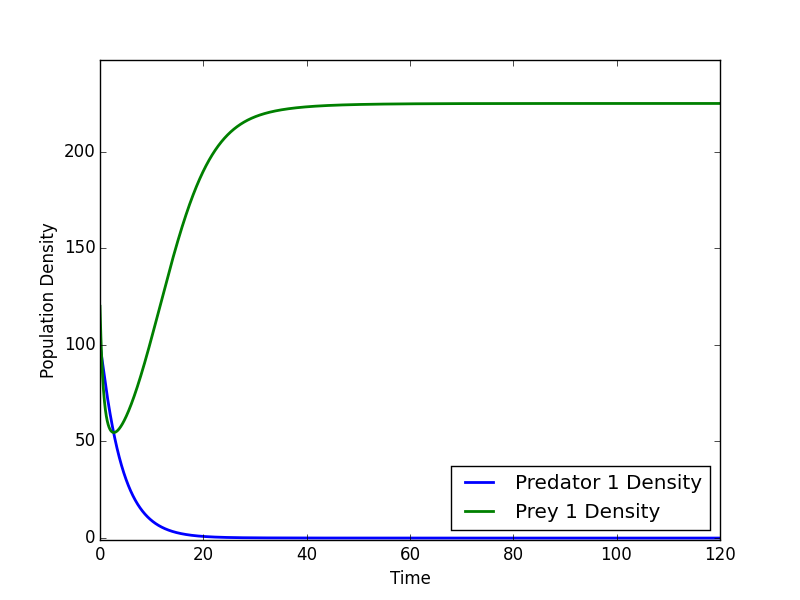
\includegraphics[width=6cm,height=4cm]{figures/1x1/constant_growth/densities_exclusion.png}
		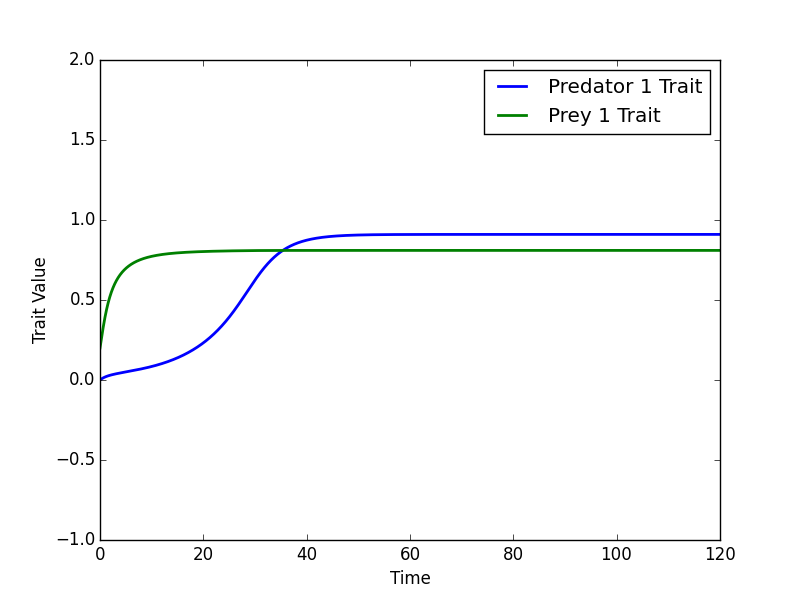
\includegraphics[width=6cm,height=4cm]{figures/1x1/constant_growth/traits_exclusion.png}
		\caption{Model 1: Exclusion Equilibrium}
		\label{fig:constant_growth_exclusion}
	\end{figure}
	\begin{figure}
		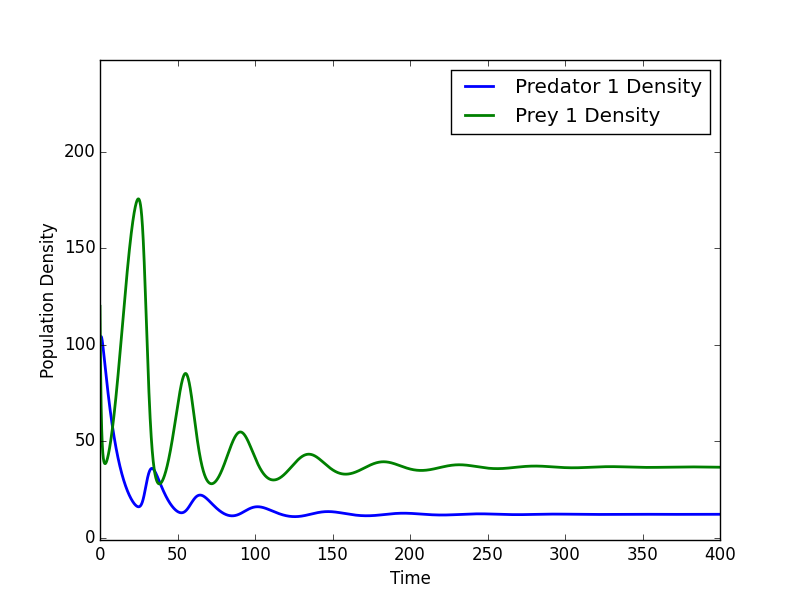
\includegraphics[width=6cm,height=4cm]{figures/1x1/constant_growth/densities_stable_coexistence.png}
		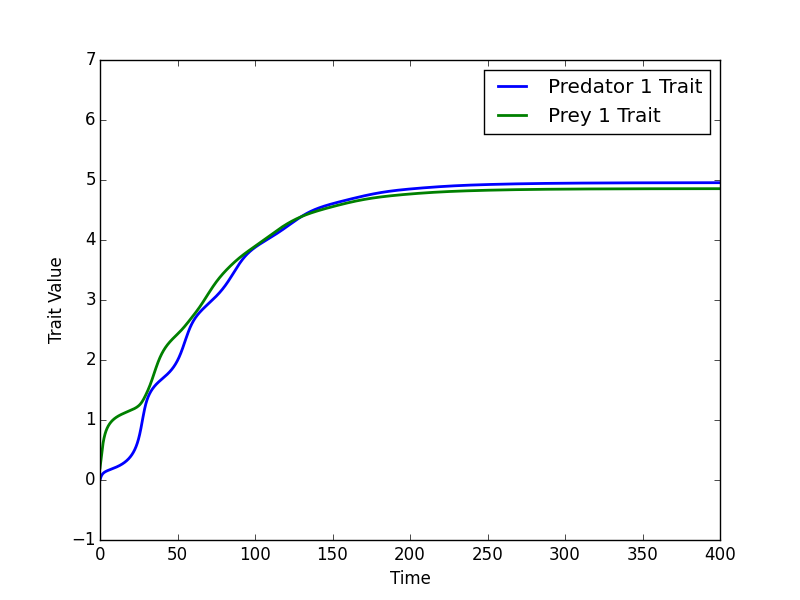
\includegraphics[width=6cm,height=4cm]{figures/1x1/constant_growth/traits_stable_coexistence.png}
		\caption{Model 1: Coexistence Equilibrium}
		\label{fig:constant_growth_coexistence_equilibrium}
	\end{figure}
	\begin{figure}
		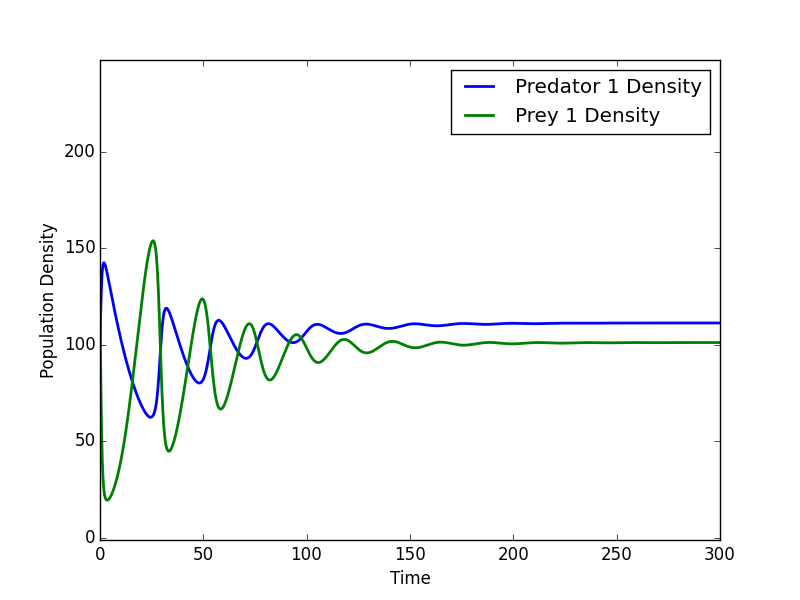
\includegraphics[width=6cm,height=4cm]{figures/1x1/constant_growth/densities_unstable_coexistence.png}
		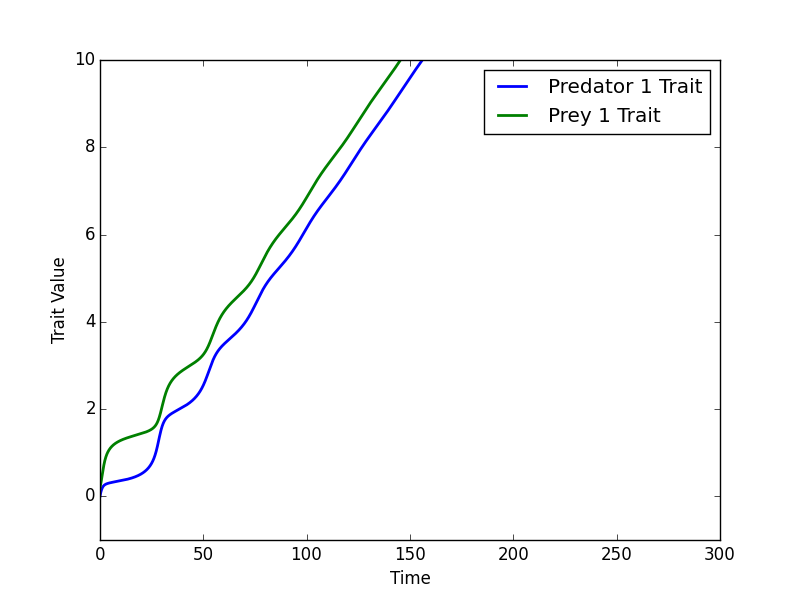
\includegraphics[width=6cm,height=4cm]{figures/1x1/constant_growth/traits_unstable_coexistence.png}
		\caption{Model 1: Non-Equilibrium Coexistence}
		\label{fig:constant_growth_non-equilibrium_coexistence}
	\end{figure}
\end{centering}


If there is only one predator species and one prey species, then (\ref{model1}) simplifies:
\begin{subequations}
	\label{MODEL1}
	\begin{align}
		\label{eq:MODEL1_A}
		\frac{dM}{dt} &= M\left[e\overline{a}(\overline{m}, \overline{n})N - d\right] \\[5px]
		\label{eq:MODEL1_B}
		\frac{dN}{dt} &= N\left[r\left(1 - \frac{N}{K}\right) - \overline{a}(\overline{m}, \overline{n})M\right] \\[5px]
		\label{eq:MODEL1_C}
		\frac{d\overline{m_i}}{dt} &= \sigma_{G}^2\frac{eN(\theta - (\overline{m} - \overline{n}))}{A}\overline{a}(\overline{m}, \overline{n}) \\[5px]
		\label{eq:MODEL1_D}
		\frac{d\overline{n_j}}{dt} &= \beta_{G}^2\frac{M(\theta - (\overline{m} - \overline{n}))}{A}\overline{a}(\overline{m}, \overline{n})
	\end{align}
\end{subequations}
There are three classifications of equilibria of (\ref{MODEL1}): extinction, exclusion, and coexistence.  There are an infinite amount of equilibrium points for each of these three classifications.  Extinction equilibria are given by
\begin{equation}
	\label{extinction_MODEL1}
	(M^*, N^*, \overline{m}^*, \overline{n}^*) = (0, 0, \mu^*, \nu^*)
\end{equation}
where $\mu^*$ and $\nu^*$ are arbitrary values.  Exclusion equilibria are given by
\begin{equation}
	\label{exclusion_MODEL1}
	(M^*, N^*, \overline{m}^*, \overline{n}^*) = (0, K, \mu^* + \theta, \mu^*)
\end{equation}
where $\mu^*$ is an arbitrary value.  Coexistence equilibria are given by
\begin{equation}
	\label{coexistence_MODEL1}
	\begin{aligned}
		(M^*, N^*, \overline{m}^*, \overline{n}^*) = \left(\frac{r\sqrt{A}}{\alpha\tau}\left(1 - \frac{N^*}{K}\right), \frac{d\sqrt{A}}{e\alpha\tau}, \mu^* + \theta, \mu^*\right)
	\end{aligned}
\end{equation}
where $\mu^*$ is an arbitrary value.  Local stability analysis (Appendix II) yields that all extinction equilibria are unstable, exclusion equilibria are asymptotically stable if
\begin{equation}
	\label{exclusion_stability_MODEL1}
	d > \frac{Ke\alpha\tau}{\sqrt{A}}
\end{equation}
and coexistence equilibria are asymptotically stable if
\begin{equation}
	\label{coexistence_stability_MODEL1}
	\frac{\sigma_G^2}{\beta_G^2} > \frac{r}{d}\left(1 - \frac{d\sqrt{A}}{Ke\alpha\tau}\right)
\end{equation}
Intuitively, exclusion is stable if the predator death rate is high enough.  Note that if (\ref{exclusion_stability_MODEL1}) holds then (\ref{coexistence_MODEL1}) is not biologically feasible ($M^* < 0$), and so even though (\ref{coexistence_stability_MODEL1}) would hold (since all parameters are assumed to be positive), it would be irrelevant.  Since $\sigma_G^2/\beta_G^2$ is the ratio of predator and prey ``speeds'' of evolution, then intuitively, coexistence is stable if the predator is ``fast'' enough at evolving in comparison to the prey.  If this happens, the predator trait value ``catches up'' to the prey trait value.  Figure \ref{fig:constant_growth_exclusion} displays a simulation that results in stable exclusion, and Figure \ref{fig:constant_growth_coexistence_equilibrium} displays a simulation that results in stable coexistence.

Since (\ref{exclusion_stability_MODEL1}) and (\ref{coexistence_stability_MODEL1}) are not equal and opposite conditions, however, there is at least one type of non-equilibrium coexistence dynamic.  Numerical simulations provide insight into these dynamics.  Figure \ref{fig:constant_growth_non-equilibrium_coexistence} depicts an evolutionary ``arms race'' between the predator and prey.  The prey has no particular optimal value, and the predator is not fast enough at evolving to catch up to the prey, so they continuously evolve in a linear fashion.  There is no stabilizing selection in this model - the prey species has no reason to stop evolving, and the predator species has no reason to stop chasing it.

\subsection{Pairwise Predator-Prey Dynamics of Model 2}
If there is only one predator species and one prey species, then (\ref{model2}) simplifies:
\begin{subequations}
	\label{MODEL2}
	\begin{align}
		\label{eq:MODEL2_A}
		\frac{dM}{dt} &= M\left[e\overline{a}(\overline{m}, \overline{n})N - d\right] \\[5px]
		\label{eq:MODEL2_B}
		\frac{dN}{dt} &= N\left[\overline{r}(\overline{n})\left(1 - \frac{N}{K}\right) - \overline{a}(\overline{m}, \overline{n})M\right] \\[5px]
		\label{eq:MODEL2_C}
		\frac{d\overline{m_i}}{dt} &= \sigma_{G}^2\frac{eN(\theta - (\overline{m} - \overline{n}))}{A}\overline{a}(\overline{m}, \overline{n}) \\[5px]
		\label{eq:MODEL2_D}
		\frac{d\overline{n}}{dt} &= \beta_{G}^2\Bigg[\overline{r}(\overline{n})\left(1 - \frac{N}{K}\right)\frac{\phi - \overline{n}}{B} + \frac{M(\theta - (\overline{m} - \overline{n}))}{A}\overline{a}(\overline{m}, \overline{n})\Bigg]
	\end{align}
\end{subequations}
Similarly to (\ref{MODEL1}), there are three classifications of equilibrium of system (\ref{MODEL2}): extinction, exclusion, and coexistence.  There are an infinite amount of equilibrium points for the extinction and exclusion classifications, but stabilizing selection provides a unique coexistence equilibrium point.  Extinction equilibria are given by (\ref{extinction_MODEL1}), and exclusion equilibria are given by (\ref{exclusion_MODEL1}).  The coexistence equilibrium point is given by
\begin{centering}
	\begin{figure}
		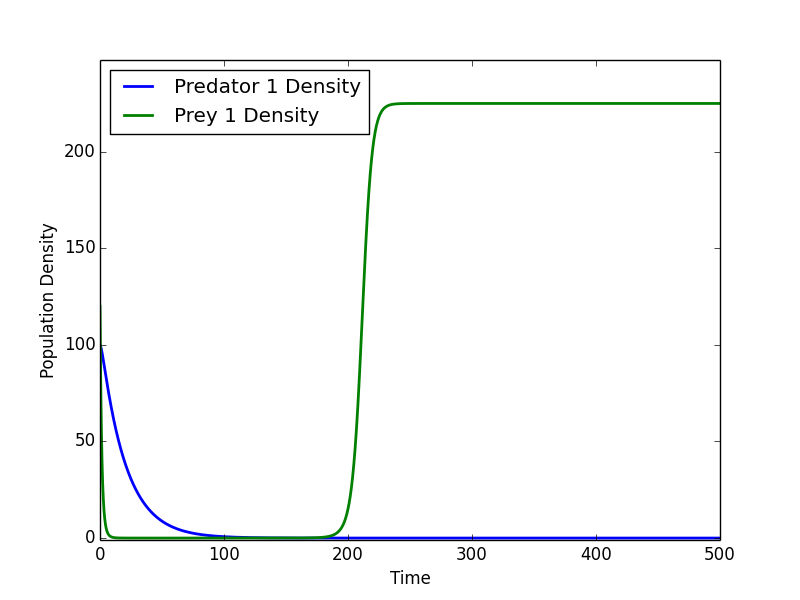
\includegraphics[width=6cm,height=4cm]{figures/1x1/variable_growth/stable_exclusion/densities.png}
		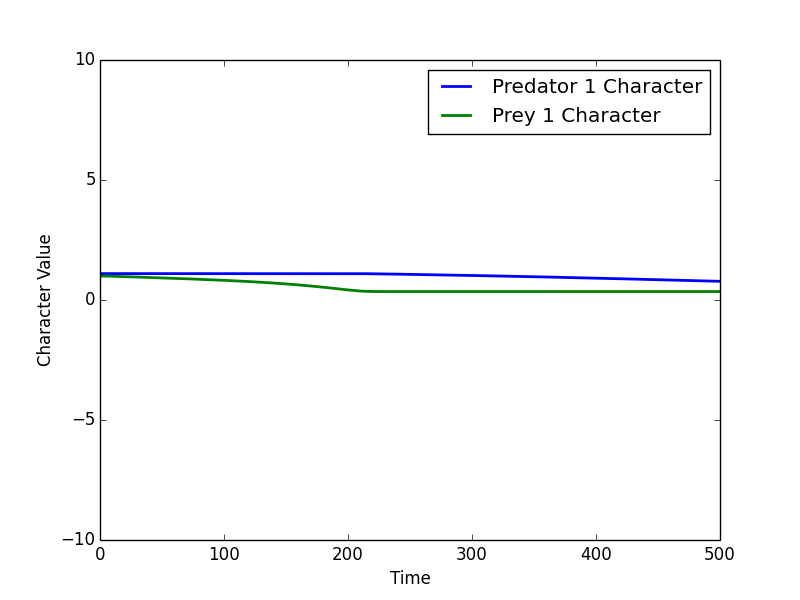
\includegraphics[width=6cm,height=4cm]{figures/1x1/variable_growth/stable_exclusion/traits.png}
		\caption{Model 2: Exclusion Equilibrium}
		\label{fig:variable_growth_exclusion}
	\end{figure}
	\begin{figure}
		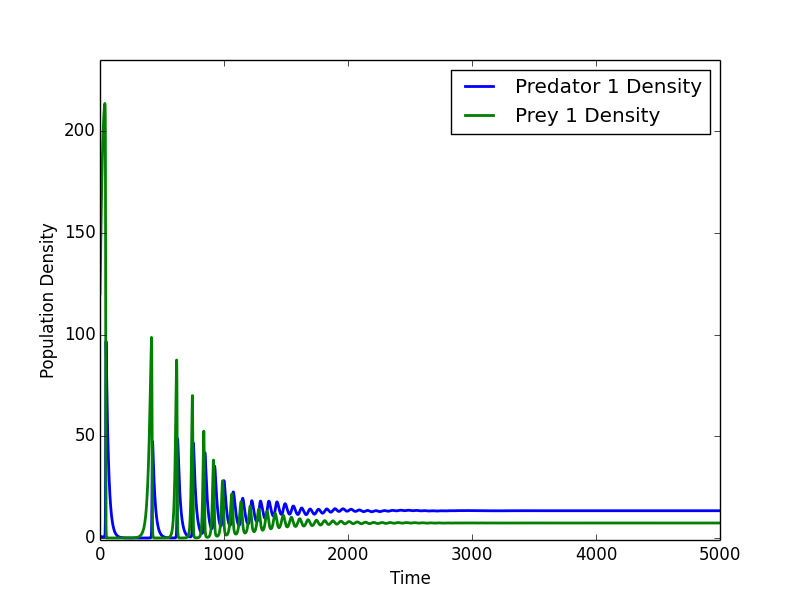
\includegraphics[width=6cm,height=4cm]{figures/1x1/variable_growth/stable_coexistence/densities.png}
		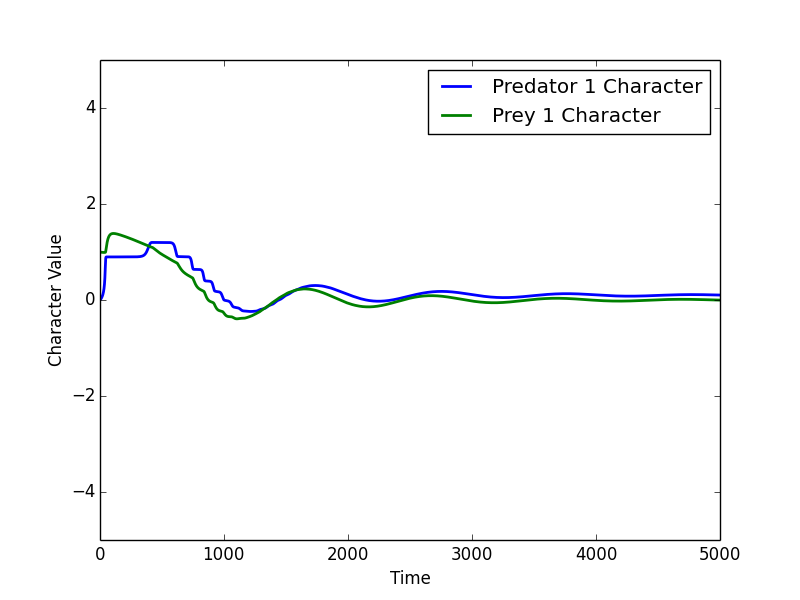
\includegraphics[width=6cm,height=4cm]{figures/1x1/variable_growth/stable_coexistence/traits.png}
		\caption{Model 2: Coexistence Equilibrium}
		\label{fig:variable_growth_coexistence_equilibrium}
	\end{figure}
	\begin{figure}
		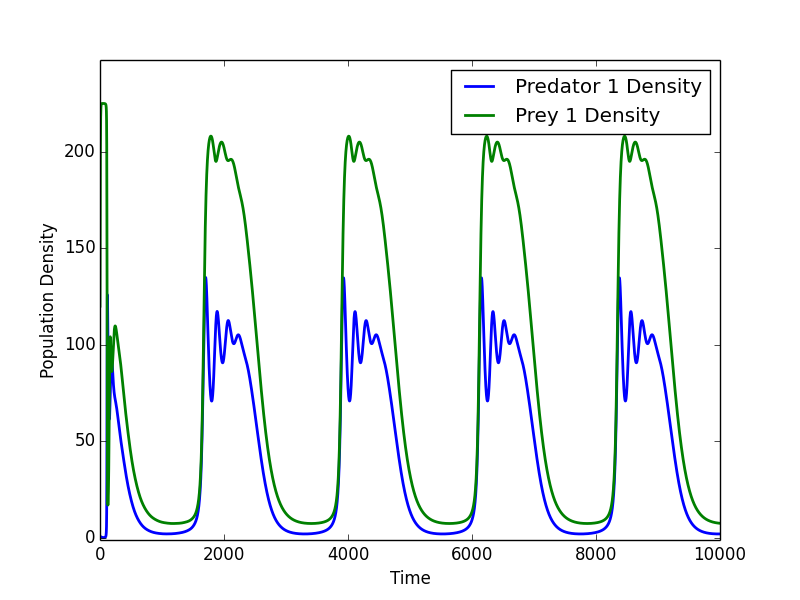
\includegraphics[width=6cm,height=4cm]{figures/1x1/variable_growth/stable_cycles/densities.png}
		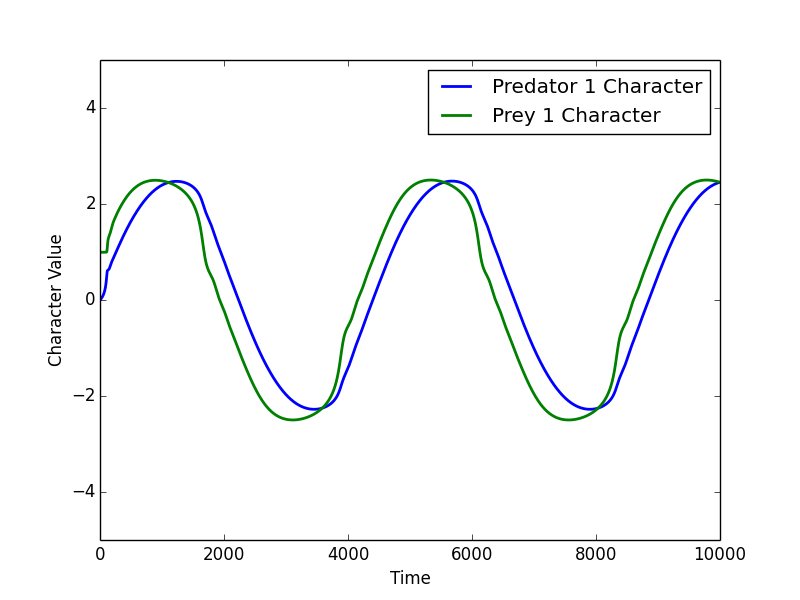
\includegraphics[width=6cm,height=4cm]{figures/1x1/variable_growth/stable_cycles/traits.png}
		\caption{Model 2: Non-Equilibrium, Cyclic Coexistence}
		\label{fig:variable_growth_stable_cycles}
	\end{figure}
\end{centering}
\begin{equation}
	\label{coexistence_MODEL2}
	\begin{aligned}
		(M^*, N^*, \overline{m}^*, \overline{n}^*) = \left(\frac{\rho\gamma\sqrt{A}}{\alpha\tau\sqrt{B}}\left(1 - \frac{N^*}{K}\right), \frac{d\sqrt{A}}{e\alpha\tau}, \phi + \theta, \phi\right)
	\end{aligned}
\end{equation}
Local stability analysis for extinction and exclusion equilibria is nearly identical to Model 1 - all extinction equilibria are unstable and exclusion equilibria are asymptotically stable if (\ref{exclusion_stability_MODEL1}) holds.  The coexistence equilibrium is asymptotically stable if
\begin{equation}
	\label{coexistence_stability_MODEL2}
	\frac{\sigma_G^2}{\beta_G^2} > \frac{\rho\gamma}{d\sqrt{B}}\left(1 - \frac{d\sqrt{A}}{Ke\alpha\tau}\right)\left(1 - \frac{A}{B}\right)
\end{equation}
Similar to Model 1, exclusion is stable if the predator death rate is high enough, and if (\ref{exclusion_stability_MODEL1}) holds then (\ref{coexistence_MODEL2}) is not biologically feasible ($M^* < 0$), and so even though (\ref{coexistence_stability_MODEL2}) may hold, it would be irrelevant.  Again, since $\sigma_G^2/\beta_G^2$ is the ratio of predator and prey ``speeds'' of evolution, then coexistence is stable only if the predator is ``fast'' enough at evolving in comparison to the prey.  Figure \ref{fig:variable_growth_exclusion} displays a simulation that results in stable exclusion, and Figure \ref{fig:variable_growth_coexistence_equilibrium} displays a simulation that results in stable coexistence.

(\ref{exclusion_stability_MODEL1}) and (\ref{coexistence_stability_MODEL2}) are not equal and opposite conditions, so there is at least one type of non-equilibrium coexistence dynamic.  Numerical simulations provide insight into these dynamics.  Figure \ref{fig:variable_growth_stable_cycles}) depicts long-term stable oscillatory dynamics.  We conjecture a unique stable limit cycle exists if neither (\ref{exclusion_stability_MODEL1}) nor (\ref{coexistence_stability_MODEL2}) hold.

We can intuitively understand these dynamics by considering the inverse effects that the evolution of the prey trait has on its own fitness.  At the same time the prey evolves its own trait value away from the predator trait value (to minimize attack rate), it must also stay close enough to its optimal trait value $\phi_j$ to maintain an adequate growth rate.  These effects nullify each other whenever the prey trait value reaches a maximum or minimum.  Immediately after the prey trait value reverses direction, the prey has double incentive to evolve toward $\phi_j$: it increases its growth rate while minimizing the predator's attack rate.  Immediately after passing through $\phi_j$, however, the inverse effects take hold, and the cycle begins again.

\pagebreak
\section{Appendices}
\subsection{Appendix 1: Derivation of Models 1 and 2}
\subsubsection{Derivation of (\ref{average_attack_rate})}
First note the following:
\begin{align*}
	\int\limits_{\mathbb{R}}\exp\left[-(ax^2 + bx + c)\right] = \sqrt{\frac{\pi}{a}}\exp\left[\frac{b^2}{4a} - c\right]
\end{align*}
\begin{align*}
	&\int\limits_{\mathbb{R}^2}a_{ij}(m_i, n_j)p(m_i, \overline{m_i})p(n_j, \overline{n_j})dm_idn_j \\
	&= \frac{\alpha_{ij}}{2\pi\sigma_i\beta_j}\int\limits_{\mathbb{R}^2}\exp\left[-\frac{((m_i - n_j) - \theta_{ij})^2}{2\tau_{ij}^2} - \frac{(m_i - \overline{m_i})^2}{2\sigma_i^2} - \frac{(n_j - \overline{n_j})^2}{2\beta_j^2}\right]dm_idn_j \\
	&= \frac{\alpha_{ij}}{2\pi\sigma_i\beta_j}\int\limits_{\mathbb{R}}\exp\left[-\frac{(n_j - \overline{n_j})^2}{2\beta_j^2}\right]\int\limits_{\mathbb{R}}\exp\left[-(am_i^2 + bm_i + c)\right]dm_idn_j
\end{align*}
where $a = \dfrac{\sigma_i^2 + \tau_{ij}^2}{2\sigma_i^2\tau_{ij}^2}$, $b = -\left(\dfrac{\sigma_i^2(n + \theta_{ij}) + \tau_{ij}^2\overline{m}}{\tau_{ij}^2\sigma_i^2}\right)$, $c = \dfrac{\sigma_i^2(n_j + \theta_{ij})^2 + \tau_{ij}^2\overline{m}^2}{2\sigma_i^2\tau_{ij}^2}$
\begin{align*}
	\implies \sqrt{\frac{\pi}{a}}\exp\left[\frac{b^2}{4a} - c\right] = \frac{\sigma_i\tau_{ij}\sqrt{2\pi}}{\sqrt{\sigma_i^2 + \tau_{ij}^2}}\exp\left[-\frac{((\overline{m} - n) - \theta_{ij})^2}{2(\sigma_i^2 + \tau_{ij}^2)}\right]
\end{align*}
Thus
\begin{align*}
	&\int\limits_{\mathbb{R}^2}a_{ij}(m_i, n_j)p(m_i, \overline{m_i})p(n_j, \overline{n_j})dm_idn_j \\
	&= \frac{\alpha_{ij}\tau_{ij}}{\beta_j\sqrt{2\pi}\sqrt{\sigma_i^2 + \tau_{ij^2}}}\int\limits_{\mathbb{R}}\exp\Bigg[-\frac{((\overline{m_i} - n_j) - \theta_{ij})^2}{2(\sigma_i^2 + \tau_{ij}^2)} - \frac{(n_j - \overline{n_j})^2}{2\beta_j^2}\Bigg]dn_j \\
	&= \frac{\alpha_{ij}\tau_{ij}}{\beta_j\sqrt{2\pi}\sqrt{\sigma_i^2 + \tau_{ij^2}}}\int\limits_{\mathbb{R}}\exp\left[-(am_i^2 + bm_i + c)\right]dn_j
\end{align*}
where $a = \dfrac{\tau_{ij}^2 + \sigma_i^2 + \beta_j^2}{2\beta_j^2(\sigma_i^2 + \tau_{ij}^2)}$, $b = -\dfrac{(\overline{m_i} - \theta_{ij})^2\beta_j^2 + (\sigma_i^2 + \tau_{ij}^2)\overline{n_j}}{\beta_j^2(\sigma_i^2 + \tau_{ij}^2)}$, and $c = \dfrac{(\overline{m_i} - \theta_{ij})^2\beta_j^2 + \overline{n}^2(\sigma_i^2 + \tau_{ij}^2)^2}{2\beta_j^2(\sigma_i^2 + \tau_{ij}^2)}$
\begin{align*}
	\implies \sqrt{\frac{\pi}{a}}&\exp\left[\frac{b^2}{4a} - c\right] = \frac{\beta_j\sqrt{2\pi}\sqrt{\sigma_i^2 + \tau_{ij}^2}}{\sqrt{\beta_j^2 + \sigma_i^2 + \tau_{ij}^2}}\exp\left[-\frac{((\overline{m} - \overline{n}) - \theta_{ij})^2}{2(\beta_j^2 + \sigma_i^2 + \tau_{ij}^2)}\right]
\end{align*}
Thus
\begin{align*}
	&\int\limits_{\mathbb{R}^2}a_{ij}(m_i, n_j)p(m_i, \overline{m_i})p(n_j, \overline{n_j})dm_idn_j = \frac{\alpha_{ij}\tau_{ij}}{\sqrt{\tau_{ij}^2 + \sigma_i^2 + \beta_j^2}}\exp{\left[-\frac{((\overline{m_i} - \overline{n_j}) - \theta_{ij})^2}{2(\tau_{ij}^2 + \sigma_i^2 + \beta_j^2)}\right]}
\end{align*}
\subsubsection{Derivation of (\ref{model_1_avg_pred_fitness})}
\begin{align*}
	\overline{W_i}(N_1, \dots, &N_u, M_i, \overline{n_1}, \dots, \overline{n_v}, \overline{m_i}) = \int\limits_{\mathbb{R}^{v+1}}^{}W_ip(m_i, \overline{m_i})\prod\limits_{j = 1}^{v}p(n_j, \overline{n_j})dm_i\prod\limits_{j = 1}^{v}dn_j \\
	&= \int\limits_{\mathbb{R}^{v+1}}^{}\left[\sum\limits_{j = 1}^{v}\left[e_{ij}a_{ij}(m_i, n_j)N_i\right] - d_i\right]p(m_i, \overline{m_i})\prod\limits_{j = 1}^{v}p(n_j, \overline{n_j})dm_i\prod\limits_{j = 1}^{v}dn_j \\
	&= \sum_{j=1}^{v}e_{ij}N_i\int\limits_{\mathbb{R}^{v+1}}^{}a_{ij}(m_i, n_j)p(m_i, \overline{m_i})\prod\limits_{j = 1}^{v}p(n_j, \overline{n_j})dm_i\prod\limits_{j = 1}^{v}dn_j \\
	&\ \ \ \ \ \ \ \ \ \ \ \ \ \ \ \ \ \ \ \ \ \ \ \ - d_i\int\limits_{\mathbb{R}^{v+1}}p(m_i, \overline{m_i})\prod\limits_{j = 1}^{v}p(n_j, \overline{n_j})dm_i\prod\limits_{j = 1}^{v}dn_j
\end{align*}
by the linearality of integrals.  Since $p(m_i, \overline{m_i})$ is independent of $n_k$ for $k = 1, \dots, v$ and $a_{ij}(m_i, n_j)$ and $p(n_j, \overline{n_j})$ are independent of $n_k$ for $k = 1, \dots, n_{j-1}, n_{j+1}, \dots, n_v$, then
\begin{align*}
	\int\limits_{\mathbb{R}^{v+1}}^{}&a_{ij}(m_i, n_j)p(m_i, \overline{m_i})\prod\limits_{j = 1}^{v}p(n_j, \overline{n_j})dm_i\prod\limits_{j = 1}^{v}dn_j \\
	&= \int\limits_{\mathbb{R}^2}a_{ij}(m_i, n_j)p(m_i, \overline{m_i})p(n_j, \overline{n_j})\left[\int\limits_{\mathbb{R}^{v-1}}\prod\limits_{\substack{k=1\\k\neq j}}^{v}p(n_k, \overline{n_k})\prod\limits_{\substack{k=1\\k\neq j}}^{v}dn_k\right]dm_idn_j
\end{align*}
However, all traits are assumed to have normal distributions, so
\begin{align*}
	\int\limits_{\mathbb{R}^{v-1}}\prod\limits_{\substack{k=1\\k\neq j}}^{v}p(n_k, \overline{n_k})\prod\limits_{\substack{k=1\\k\neq j}}^{v}dn_k = 1
\end{align*}
Thus
\begin{align*}
	\int\limits_{\mathbb{R}^{v+1}}^{}a_{ij}(m_i, n_j)p(m_i, \overline{m_i})\prod\limits_{j = 1}^{v}p(n_j, \overline{n_j})dm_i\prod\limits_{j = 1}^{v}dn_j &= \int\limits_{\mathbb{R}^2}a_{ij}(m_i, n_j)p(m_i, \overline{m_i})p(n_j, \overline{n_j})dm_idn_j \\
	&= \overline{a_{ij}}(\overline{m_i}, \overline{n_j})
\end{align*}
and
\begin{align*}
	d_i\left(\int\limits_{\mathbb{R}^{v+1}}p(m_i, \overline{m_i})\prod\limits_{j = 1}^{v}p(n_j, \overline{n_j})dm_i\prod\limits_{j = 1}^{v}dn_j\right) = d_i
\end{align*}
Thus,
\begin{align*}
	\overline{W_i}(N_1, \dots, &N_u, M_i, \overline{n_1}, \dots, \overline{n_v}, \overline{m_i}) = \sum\limits_{j = 1}^{v}\left[e_{ij}\overline{a_{ij}}(\overline{m_i}, \overline{n_j})N_i\right] - d_i
\end{align*}
\subsubsection{Derivation of (\ref{model_1_avg_prey_fitness})}
\begin{align*}
	\overline{Y_j}(N_j, M_1, \dots, &M_v, \overline{n_j}, \overline{m_1}, \dots, \overline{m_v}) = \int\limits_{\mathbb{R}^{u+1}}^{}Y_jp(n_j, \overline{n_j})\prod\limits_{i = 1}^{u}p(m_i, \overline{m_i})dn_j\prod\limits_{i = 1}^{u}dm_i \\
	&= \int\limits_{\mathbb{R}^{u+1}}\left[r_j\left(1 - \frac{N_j}{K_j}\right) - \sum\limits_{i = 1}^{u}\left[a_{ij}(m_i, n_j)M_i\right]\right]p(n_j, \overline{n_j})\prod\limits_{i = 1}^{u}p(m_i, \overline{m_i})dn_j\prod\limits_{i = 1}^{u}dm_i \\
	&= r_j\left(1 - \frac{N_j}{K_j}\right)\int\limits_{\mathbb{R}^{u+1}}p(n_j, \overline{n_j})\prod\limits_{i = 1}^{u}p(m_i, \overline{m_i})dn_j\prod\limits_{i = 1}^{u}dm_i \\
	&\ \ \ \ \ \ \ \ \ \ \ \ \ \ \ - \sum\limits_{i=1}^{u}M_i\int\limits_{\mathbb{R}^{u+1}}a_{ij}(m_i, n_j)p(n_j, \overline{n_j})\prod\limits_{i = 1}^{u}p(m_i, \overline{m_i})dn_j\prod\limits_{i = 1}^{u}dm_i
\end{align*}
Similary to the derivation of (\ref{model_1_avg_pred_fitness}),
\begin{align*}
	r_j\left(1 - \frac{N_j}{K_j}\right)\left(\ \int\limits_{\mathbb{R}^{u+1}}p(n_j, \overline{n_j})\prod\limits_{i = 1}^{u}p(m_i, \overline{m_i})dn_j\prod\limits_{i = 1}^{u}dm_i\right) = r_j\left(1 - \frac{N_j}{K_j}\right)
\end{align*}
and
\begin{align*}
	\int\limits_{\mathbb{R}^{u+1}}a_{ij}(m_i, n_j)p(n_j, \overline{n_j})\prod\limits_{i = 1}^{u}p(m_i, \overline{m_i})dn_j\prod\limits_{i = 1}^{u}dm_i = \overline{a_{ij}}(\overline{m_i}, \overline{n_j})
\end{align*}
Thus,
\begin{align*}
	\overline{Y_j}(N_j, M_1, \dots, &M_v, \overline{n_j}, \overline{m_1}, \dots, \overline{m_v}) = r_j\left(1 - \frac{N_j}{K_j}\right) - \sum\limits_{i = 1}^{u}\left[\overline{a_{ij}}(\overline{m_i}, \overline{n_j})M_i\right]
\end{align*}
\subsubsection{Derivation of (\ref{average_growth_rate})}
\begin{align*}
	\overline{r_j}(\overline{n_j}) &= \int\limits_{\mathbb{R}}^{}r_j(n_j)p(n_j, \overline{n_j})dn_j \\
	&= \int\limits_{\mathbb{R}}\left(\rho_j\exp\left[-\frac{(n_j - \phi_j)^2}{2\gamma_j^2}\right]\right)\left(\frac{1}{\sqrt{2\pi\beta_j^2}}\exp\left[-\frac{(n_j - \overline{n_j})^2}{2\beta_j^2}\right]\right)dn_j \\
	&= \frac{\rho_j}{\beta_j\sqrt{2\pi}}\int\limits_{\mathbb{R}}\exp\left[-(an_j^2 + bn_j + c)\right]dn_j
\end{align*}
where $a = \dfrac{\beta_j^2 + \gamma_j^2}{2\beta_j^2\gamma_j^2}$, $b = -\left(\dfrac{\phi_j\beta_j^2 + \overline{n_j}\gamma_j^2}{\beta_j^2\gamma_j^2}\right)$, and $c = \dfrac{\phi_j^2\beta_j^2 + \overline{n_j}^2\gamma_j^2}{2\beta_j^2\gamma_j^2}$
\begin{align*}
	\implies \sqrt{\frac{\pi}{a}}\exp\left[\frac{b^2}{4a} - c\right] &= \frac{\beta_j\gamma_j\sqrt{2\pi}}{\sqrt{\beta_j^2 + \gamma_j^2}}\exp\left[-\frac{(\overline{n_j} - \phi_j)^2}{2(\beta_j^2 + \gamma_j^2)}\right] \\
	\implies \overline{r_j}(n_j) &= \frac{\rho_j\gamma_j}{\sqrt{B_j}}\exp\left[-\frac{(\overline{n_j} - \phi_j)^2}{2B_j}\right]
\end{align*}
\subsubsection{Derivation of (\ref{model_2_avg_prey_fitness})}
\begin{align*}
	\overline{Y_j}(N_j, M_1, \dots, &M_v, \overline{n_j}, \overline{m_1}, \dots, \overline{m_v}) = \int\limits_{\mathbb{R}^{u+1}}^{}Y_jp(n_j, \overline{n_j})\prod\limits_{i = 1}^{u}p(m_i, \overline{m_i})dn_j\prod\limits_{i = 1}^{u}dm_i \\
	&= \int\limits_{\mathbb{R}^{u+1}}\left[r_j(n_j)\left(1 - \frac{N_j}{K_j}\right) - \sum\limits_{i = 1}^{u}\left[a_{ij}(m_i, n_j)M_i\right]\right]p(n_j, \overline{n_j})\prod\limits_{i = 1}^{u}p(m_i, \overline{m_i})dn_j\prod\limits_{i = 1}^{u}dm_i \\
	&= \left(1 - \frac{N_j}{K_j}\right)\int\limits_{\mathbb{R}^{u+1}}r_j(n_j)p(n_j, \overline{n_j})\prod\limits_{i = 1}^{u}p(m_i, \overline{m_i})dn_j\prod\limits_{i = 1}^{u}dm_i \\
	&\ \ \ \ \ \ \ \ \ \ \ \ \ \ \ - \sum\limits_{i=1}^{u}M_i\int\limits_{\mathbb{R}^{u+1}}a_{ij}(m_i, n_j)p(n_j, \overline{n_j})\prod\limits_{i = 1}^{u}p(m_i, \overline{m_i})dn_j\prod\limits_{i = 1}^{u}dm_i
\end{align*}
Similary to the derivation of (\ref{model_1_avg_pred_fitness}), since $r_j(n_j)$ and $p(n_j, \overline{n_j})$ are not dependent on $n_k$ for $k = 1, \dots, \j-1, \j+1, \dots, v$, then 
\begin{align*}
	\int\limits_{\mathbb{R}^{u+1}}^{}r_j(n_j)p(m_i, \overline{m_i})&\prod\limits_{j = 1}^{v}p(n_j, \overline{n_j})dm_i\prod\limits_{j = 1}^{v}dn_j \\
	&= \int\limits_{\mathbb{R}}r_j(n_j)p(n_j, \overline{n_j})\left[\int\limits_{\mathbb{R}^{u}}p(m_i, \overline{m_i})\prod\limits_{\substack{k=1\\k\neq j}}^{v}p(n_k, \overline{n_k})dm_i\prod\limits_{\substack{k=1\\k\neq j}}^{v}dn_k\right]dn_j \\
	&= \int\limits_{\mathbb{R}}r_j(n_j)p(n_j, \overline{n_j})dn_j \\
	&= \overline{r_j}(\overline{n_j})
\end{align*}
and
\begin{align*}
	\int\limits_{\mathbb{R}^{u+1}}a_{ij}(m_i, n_j)p(n_j, \overline{n_j})\prod\limits_{i = 1}^{u}p(m_i, \overline{m_i})dn_j\prod\limits_{i = 1}^{u}dm_i = \overline{a_{ij}}(\overline{m_i}, \overline{n_j})
\end{align*}
Thus,
\begin{align*}
	\overline{Y_j}(N_j, M_1, \dots, &M_v, \overline{n_j}, \overline{m_1}, \dots, \overline{m_v}) = \overline{r_j}(\overline{n_j})\left(1 - \frac{N_j}{K_j}\right) - \sum\limits_{i = 1}^{u}\left[\overline{a_{ij}}(\overline{m_i}, \overline{n_j})M_i\right]
\end{align*}

\pagebreak
\subsection{Appendix 2: Equilibria and Local Stability Analysis of (\ref{MODEL1})}
\begin{align*}
	f_1 = \frac{dM}{dt} &= M\left[e\overline{a}(\overline{m}, \overline{n})N - d\right] \\[5px]
	f_2 = \frac{dN}{dt} &= N\left[r\left(1 - \frac{N}{K}\right) - \overline{a}(\overline{m}, \overline{n})M\right] \\[5px]
	f_3 = \frac{d\overline{m}}{dt} &= \sigma_{G}^2\frac{eN(\theta - (\overline{m} - \overline{n}))}{A}\overline{a}(\overline{m}, \overline{n}) \\[5px]
	f_4 = \frac{d\overline{n}}{dt} &= \beta_{G}^2\frac{M(\theta - (\overline{m} - \overline{n}))}{A}\overline{a}(\overline{m}, \overline{n})
\end{align*}
\begin{align*}
	\begin{array}{ccccc}
		f_1 = 0 \implies& M = 0 \ \ \ &\text{or}&\ \ \ N = \dfrac{d}{e\overline{a}(\overline{m}, \overline{n})} \\[10px]
		f_2 = 0 \implies& N = 0 \ \ \ &\text{or}&\ \ \ M = \dfrac{r}{\overline{a}(\overline{m}, \overline{n})}\left(1 - \dfrac{N}{K}\right) \\[10px]
		f_3 = 0 \implies& N = 0 \ \ \ &\text{or}&\ \ \ \overline{m} - \overline{n} = \theta \\[10px]
		f_4 = 0 \implies& M = 0 \ \ \ &\text{or}&\ \ \ \overline{m} - \overline{n} = \theta
	\end{array}
\end{align*}
Clearly, $M = N = 0$ satisfies equilibrium, and $\overline{m}$ and $\overline{n}$ are arbitrary.  This gives the extinction equilibria.  Suppose $M = 0$ but $N \neq 0$.  Then $f_2 = 0 \implies N = K$ and $f_3 = 0 \implies \overline{m} - \overline{n} = \theta$.  This gives the exclusion equilibria.  Supposing $M \neq 0$ and $N \neq 0$, then $f_3 = f_4 = 0 \implies \overline{m} - \overline{n} = \theta \implies \overline{a}(\overline{m}, \overline{n}) = \frac{\alpha\tau}{\sqrt{A}} \implies N = \frac{d\sqrt{A}}{e\alpha\tau} \implies M = \frac{r\sqrt{A}}{\alpha\tau}\left(1 - \frac{\sqrt{A}}{Ke\alpha\tau}\right)$.  By exhaustion, this gives the only other set of equilibria: the coexistence equilibria.

To solve for local stability conditions, we find the eigenvalues of the community matrix evaluated at each equilbrium point.  First, note the partial derivatives of $f_1$, $f_2$, $f_3$, and $f_4$:
\begin{align*}
	\frac{\partial f_1}{\partial M} &= e\overline{a}(\overline{m}, \overline{n})N - d\\[5px]
	\frac{\partial f_1}{\partial N} &= Me\overline{a}(\overline{m}, \overline{n})\\[5px]
	\frac{\partial f_1}{\partial \overline{m}} &= \frac{MNe(\theta - (\overline{m} - \overline{n}))}{A}\overline{a}(\overline{m}, \overline{n}) \\[5px]
	\frac{\partial f_1}{\partial \overline{n}} &= \frac{MNe((\overline{m} - \overline{n}) - \theta)}{A}\overline{a}(\overline{m}, \overline{n})
\end{align*}
\begin{align*}
	\frac{\partial f_2}{\partial M} &= -N\overline{a}(\overline{m}, \overline{n}) \\[5px]
	\frac{\partial f_2}{\partial N} &= r\left(1 - \frac{2N}{K}\right) - M\overline{a}(\overline{m}, \overline{n})\\[5px]
	\frac{\partial f_2}{\partial \overline{m}} &= -\frac{MN(\theta - (\overline{m} - \overline{n}))}{A}\overline{a}(\overline{m}, \overline{n}) \\[5px]
	\frac{\partial f_2}{\partial \overline{n}} &= -\frac{MN((\overline{m} - \overline{n}) - \theta)}{A}\overline{a}(\overline{m}, \overline{n})
\end{align*}
\begin{align*}
	\frac{\partial f_3}{\partial M} &= 0 \\[5px]
	\frac{\partial f_3}{\partial N} &= \frac{\sigma_{G}^2e}{A}\overline{a}(\overline{m}, \overline{n})(\theta - (\overline{m} - \overline{n})) \\[5px]
	\frac{\partial f_3}{\partial \overline{m}} &= \frac{\sigma_G^2eN}{A}\overline{a}(\overline{m}, \overline{n})\left(\frac{(\theta - (\overline{m} - \overline{n}))^2}{A} - 1\right)\\[5px]
	\frac{\partial f_3}{\partial \overline{n}} &= \frac{\sigma_G^2eN}{A}\overline{a}(\overline{m}, \overline{n})\left(1 - \frac{(\theta - (\overline{m} - \overline{n}))^2}{A}\right)
\end{align*}
\begin{align*}
	\frac{\partial f_4}{\partial M} &= \frac{\beta_{G}^2}{A}\overline{a}(\overline{m}, \overline{n})(\theta - (\overline{m} - \overline{n})) \\[5px]
	\frac{\partial f_4}{\partial N} &= 0 \\[5px]
	\frac{\partial f_4}{\partial \overline{m}} &= \frac{\beta_G^2M}{A}\overline{a}(\overline{m}, \overline{n})\left(\frac{(\theta - (\overline{m} - \overline{n}))^2}{A} - 1\right)\\[5px]
	\frac{\partial f_4}{\partial \overline{n}} &= \frac{\beta_G^2M}{A}\overline{a}(\overline{m}, \overline{n})\left(1 - \frac{(\theta - (\overline{m} - \overline{n}))^2}{A}\right)
\end{align*}
Let the extinction, exclusion, and coexistence equilibrium be denoted as
\begin{align*}
	E_{\text{ext}} = (M^*, N^*, \overline{m}^*, \overline{n}^*) &= (0, 0, \mu^*, \nu^*) \\
	E_{\text{excl}} = (M^*, N^*, \overline{m}^*, \overline{n}^*) &= (0, K, \mu^* + \theta, \mu^*) \\
	E_{\text{coex}} = (M^*, N^*, \overline{m}^*, \overline{n}^*) &= \left(\frac{r\sqrt{A}}{\alpha\tau}\left(1 - \frac{N^*}{K}\right), \frac{d\sqrt{A}}{e\alpha\tau}, \mu^* + \theta, \mu^*\right)
\end{align*}
Then denote $J^*|_{E_{\text{ext}}}$, $J^*|_{E_{\text{excl}}}$, and $J^*|_{E_{\text{coex}}}$ as the community matrices evaluated at those points.
\begin{align*}
	J^*|_{E_{\text{ext}}} &= \left(\begin{array}{cccc}
		\dfrac{\partial f_1}{\partial M}\Big|_{E_{\text{ext}}} & \dfrac{\partial f_1}{\partial N}\Big|_{E_{\text{ext}}} & \dfrac{\partial f_1}{\partial \overline{m}}\Big|_{E_{\text{ext}}} & \dfrac{\partial f_1}{\partial \overline{n}}\Big|_{E_{\text{ext}}} \\[10px]
		\dfrac{\partial f_2}{\partial M}\Big|_{E_{\text{ext}}} & \dfrac{\partial f_2}{\partial N}\Big|_{E_{\text{ext}}} & \dfrac{\partial f_2}{\partial \overline{m}}\Big|_{E_{\text{ext}}} & \dfrac{\partial f_2}{\partial \overline{n}}\Big|_{E_{\text{ext}}} \\[10px]
		\dfrac{\partial f_3}{\partial M}\Big|_{E_{\text{ext}}} & \dfrac{\partial f_3}{\partial N}\Big|_{E_{\text{ext}}} & \dfrac{\partial f_3}{\partial \overline{m}}\Big|_{E_{\text{ext}}} & \dfrac{\partial f_3}{\partial \overline{n}}\Big|_{E_{\text{ext}}} \\[10px]
		\dfrac{\partial f_4}{\partial M}\Big|_{E_{\text{ext}}} & \dfrac{\partial f_4}{\partial N}\Big|_{E_{\text{ext}}} & \dfrac{\partial f_4}{\partial \overline{m}}\Big|_{E_{\text{ext}}} & \dfrac{\partial f_4}{\partial \overline{n}}\Big|_{E_{\text{ext}}}
	\end{array}\right) \\
	&= \left(\begin{array}{cccc}
		-d & 0 & 0 & 0 \\
		0 & r & 0 & 0 \\
		0 & \frac{\sigma_{G}^2e(\theta - (\mu^* - \nu^*))}{A}\overline{a}(\mu^*, \nu^*) & 0 & 0 \\
		\frac{\beta_{G}^2(\theta - (\mu^* - \nu^*))}{A}\overline{a}(\mu^*, \nu^*) & 0 & 0 & 0
	\end{array}\right)
\end{align*}
This is an upper-triangular matrix, and thus the eigenvalues are the entries on the main diagonal: $-d$, $r$, and $0$.  Since one of the eigenvalues, namely $r$, is positive, the $E_{\text{ext}}$ is locally unstable.
\begin{align*}
	J^*|_{E_{\text{excl}}} &= \left(\begin{array}{cccc}
		\dfrac{\partial f_1}{\partial M}\Big|_{E_{\text{excl}}} & \dfrac{\partial f_1}{\partial N}\Big|_{E_{\text{excl}}} & \dfrac{\partial f_1}{\partial \overline{m}}\Big|_{E_{\text{excl}}} & \dfrac{\partial f_1}{\partial \overline{n}}\Big|_{E_{\text{excl}}} \\[10px]
		\dfrac{\partial f_2}{\partial M}\Big|_{E_{\text{excl}}} & \dfrac{\partial f_2}{\partial N}\Big|_{E_{\text{excl}}} & \dfrac{\partial f_2}{\partial \overline{m}}\Big|_{E_{\text{excl}}} & \dfrac{\partial f_2}{\partial \overline{n}}\Big|_{E_{\text{excl}}} \\[10px]
		\dfrac{\partial f_3}{\partial M}\Big|_{E_{\text{excl}}} & \dfrac{\partial f_3}{\partial N}\Big|_{E_{\text{excl}}} & \dfrac{\partial f_3}{\partial \overline{m}}\Big|_{E_{\text{excl}}} & \dfrac{\partial f_3}{\partial \overline{n}}\Big|_{E_{\text{excl}}} \\[10px]
		\dfrac{\partial f_4}{\partial M}\Big|_{E_{\text{excl}}} & \dfrac{\partial f_4}{\partial N}\Big|_{E_{\text{excl}}} & \dfrac{\partial f_4}{\partial \overline{m}}\Big|_{E_{\text{excl}}} & \dfrac{\partial f_4}{\partial \overline{n}}\Big|_{E_{\text{excl}}}
	\end{array}\right) \\
	&= \left(\begin{array}{cccc}
		\frac{Ke\alpha\tau}{\sqrt{A}} - d & 0 & 0 & 0 \\
		-\frac{K\alpha\tau}{\sqrt{A}} & -r & 0 & 0 \\
		0 & 0 & -\frac{\sigma_G^2Ke\alpha\tau}{A^{3/2}} & \frac{\sigma_G^2Ke\alpha\tau}{A^{3/2}} \\
		0 & 0 & 0 & 0
	\end{array}\right)
\end{align*}
The eigenvalues are $\frac{Ke\alpha\tau}{\sqrt{A}} - d$, $-r$ and $-\frac{\sigma_G^2Ke\alpha\tau}{A^{3/2}}$, $0$.  (The eigenvalues are easily computable by swapping the third and fourth rows and columns to obtain an upper-triangular matrix).  All of these are non-positive if (\ref{exclusion_stability_MODEL1}) holds.
\begin{align*}
	J^*|_{E_{\text{coex}}} &= \left(\begin{array}{cccc}
		\dfrac{\partial f_1}{\partial M}\Big|_{E_{\text{coex}}} & \dfrac{\partial f_1}{\partial N}\Big|_{E_{\text{coex}}} & \dfrac{\partial f_1}{\partial \overline{m}}\Big|_{E_{\text{coex}}} & \dfrac{\partial f_1}{\partial \overline{n}}\Big|_{E_{\text{coex}}} \\[10px]
		\dfrac{\partial f_2}{\partial M}\Big|_{E_{\text{coex}}} & \dfrac{\partial f_2}{\partial N}\Big|_{E_{\text{coex}}} & \dfrac{\partial f_2}{\partial \overline{m}}\Big|_{E_{\text{coex}}} & \dfrac{\partial f_2}{\partial \overline{n}}\Big|_{E_{\text{coex}}} \\[10px]
		\dfrac{\partial f_3}{\partial M}\Big|_{E_{\text{coex}}} & \dfrac{\partial f_3}{\partial N}\Big|_{E_{\text{coex}}} & \dfrac{\partial f_3}{\partial \overline{m}}\Big|_{E_{\text{coex}}} & \dfrac{\partial f_3}{\partial \overline{n}}\Big|_{E_{\text{coex}}} \\[10px]
		\dfrac{\partial f_4}{\partial M}\Big|_{E_{\text{coex}}} & \dfrac{\partial f_4}{\partial N}\Big|_{E_{\text{coex}}} & \dfrac{\partial f_4}{\partial \overline{m}}\Big|_{E_{\text{coex}}} & \dfrac{\partial f_4}{\partial \overline{n}}\Big|_{E_{\text{coex}}}
	\end{array}\right) \\
	&= \left(\begin{array}{cccc}
		0 & er\left(1 - \frac{N^*}{K}\right) & 0 & 0 \\
		-\frac{d}{e} & -\frac{rN^*}{K} & 0 & 0 \\
		0 & 0 & -\frac{\sigma_G^2d}{A} & \frac{\sigma_G^2d}{A} \\
		0 & 0 & -\frac{\beta_G^2r}{A}\left(1 - \frac{N^*}{K}\right) & \frac{\beta_G^2r}{A}\left(1 - \frac{N^*}{K}\right)
	\end{array}\right)
\end{align*}
This is a block diagonal matrix, and so the eigenvalues can be calculated by finding the eigenvalues of each block.
\begin{align*}
	J_1 = \left(\begin{array}{cc}
		0 & er\left(1 - \frac{N^*}{K}\right)\\
		-\frac{d}{e} & -\frac{rN^*}{K}
	\end{array}\right)\ \ \ \ \text{and}\ \ \ \ J_2 = \left(\begin{array}{cc}
		-\frac{\sigma_G^2d}{A} & \frac{\sigma_G^2d}{A} \\
        -\frac{\beta_G^2r}{A}\left(1 - \frac{N^*}{K}\right) & \frac{\beta_G^2r}{A}\left(1 - \frac{N^*}{K}\right)
	\end{array}\right)
\end{align*}
The eigenvalues of $J_1$ are
\begin{align*}
	\lambda_{1,2} = \frac{1}{2}\left[-\frac{rN^*}{K} \pm \sqrt{\left(\frac{rN^*}{K}\right)^2 - 4rd\left(1 - \frac{N^*}{K}\right)}\ \right]
\end{align*}
Since $N^* < K$, $\sqrt{\left(\frac{rN^*}{K}\right)^2 - 4rd\left(1 - \frac{N^*}{K}\right)} < \left|\frac{rN^*}{K}\right|$, and thus $\text{Re}(\lambda_{1,2}) < 0$. \\

\noindent The eigenvalues of $J_2$ are
\begin{align*}
	\lambda_{3,4} = \frac{1}{2}\left[-\left(\frac{d\sigma_G^2 - r\beta_G^2\left(1 - \dfrac{N^*}{K}\right)}{A}\right) \pm \sqrt{\Delta}\right]
\end{align*}
where
\begin{align*}
	\Delta = \left(\frac{d\sigma_G^2 - r\beta_G^2\left(1 - \dfrac{N^*}{K}\right)}{A}\right)^2 - \left(\frac{4rd\sigma_G^2\beta_G^2\left(1 - \dfrac{N^*}{K}\right)}{A^2}\right)
\end{align*}
Again, since $N^* < K$, $\sqrt{\Delta} < \left|\dfrac{d\sigma_G^2 - r\beta_G^2\left(1 - \frac{N^*}{K}\right)}{A}\right|$, and thus $\text{Re}(\lambda_{3,4}) < 0$ if and only if (\ref{coexistence_stability_MODEL1}) holds.

\pagebreak
\subsection{Appendix 3: Equilibria and Local Stability Analysis of (\ref{MODEL2})}
\begin{align*}
	f_1 = \frac{dM}{dt} &= M\left[e\overline{a}(\overline{m}, \overline{n})N - d\right] \\[5px]
	f_2 = \frac{dN}{dt} &= N\left[\overline{r}(\overline{n})\left(1 - \frac{N}{K}\right) - \overline{a}(\overline{m}, \overline{n})M\right] \\[5px]
	f_3 = \frac{d\overline{m}}{dt} &= \sigma_{G}^2\frac{eN(\theta - (\overline{m} - \overline{n}))}{A}\overline{a}(\overline{m}, \overline{n}) \\[5px]
	f_4 = \frac{d\overline{n}}{dt} &= \beta_{G}^2\Bigg[\overline{r}(\overline{n})\left(1 - \frac{N}{K}\right)\frac{\phi - \overline{n}}{B} + \frac{M(\theta - (\overline{m} - \overline{n}))}{A}\overline{a}(\overline{m}, \overline{n})\Bigg]
\end{align*}
\begin{align*}
	\begin{array}{cccrl}
		f_1 = 0 \implies& M = 0 \ \ \ &\text{or}&\ \ \ N &= \dfrac{d}{e\overline{a}(\overline{m}, \overline{n})} \\[10px]
		f_2 = 0 \implies& N = 0 \ \ \ &\text{or}&\ \ \ M &= \dfrac{\overline{r}(\overline{n})}{\overline{a}(\overline{m}, \overline{n})}\left(1 - \dfrac{N}{K}\right) \\[10px]
		f_3 = 0 \implies& N = 0 \ \ \ &\text{or}&\ \ \ \overline{m} - \overline{n} &= \theta \\[10px]
		f_4 = 0 \implies& M = 0 \ \ \ &\text{or}&\ \ \ \overline{r}(\overline{n})\left(1 - \dfrac{N}{K}\right)\dfrac{\phi - \overline{n}}{B} &= \dfrac{M((\overline{m} - \overline{n}) - \theta)}{A}\overline{a}(\overline{m}, \overline{n})
	\end{array}
\end{align*}
Clearly, $M = N = 0$ satisfies equilibrium, and $\overline{m}$ and $\overline{n}$ are arbitrary.  This gives the extinction equilibria.  Suppose $M = 0$ but $N \neq 0$.  Then $f_2 = 0 \implies N = K$ and $f_3 = 0 \implies \overline{m} - \overline{n} = \theta$.  This gives the exclusion equilibria.  Supposing $M \neq 0$ and $N \neq 0$, then $f_3 = 0 \implies \overline{m} - \overline{n} = \theta \implies \overline{a}(\overline{m}, \overline{n}) = \frac{\alpha\tau}{\sqrt{A}} \implies N = \frac{d\sqrt{A}}{e\alpha\tau}$.  Since $\overline{m} - \overline{n} = \theta$, then $f_4 = 0 \implies \overline{n} = \phi$ or $N = K$.  But if $N = K$, then $f_2 = 0 \implies M = 0$, a contradiction.  Thus $\overline{n} = \phi$, which implies $\overline{m} = \phi + \theta$ and $M = \frac{\rho\gamma\sqrt{A}}{\alpha\tau\sqrt{B}}\left(1 - \frac{\sqrt{A}}{Ke\alpha\tau}\right)$.  By exhaustion, this gives the only other equilibrium: the coexistence equilibrium point.

To solve for local stability conditions, we find the eigenvalues of the community matrix evaluated at each equilbrium point.  First, note the partial derivatives of $f_1$, $f_2$, $f_3$, and $f_4$:
\begin{align*}
	\frac{\partial f_1}{\partial M} &= e\overline{a}(\overline{m}, \overline{n})N - d\\[5px]
	\frac{\partial f_1}{\partial N} &= Me\overline{a}(\overline{m}, \overline{n})\\[5px]
	\frac{\partial f_1}{\partial \overline{m}} &= \frac{MNe(\theta - (\overline{m} - \overline{n}))}{A}\overline{a}(\overline{m}, \overline{n}) \\[5px]
	\frac{\partial f_1}{\partial \overline{n}} &= \frac{MNe((\overline{m} - \overline{n}) - \theta)}{A}\overline{a}(\overline{m}, \overline{n})
\end{align*}
\begin{align*}
	\frac{\partial f_2}{\partial M} &= -N\overline{a}(\overline{m}, \overline{n}) \\[5px]
	\frac{\partial f_2}{\partial N} &= \overline{r}(\overline{n})\left(1 - \frac{2N}{K}\right) - M\overline{a}(\overline{m}, \overline{n})\\[5px]
	\frac{\partial f_2}{\partial \overline{m}} &= -\frac{MN(\theta - (\overline{m} - \overline{n}))}{A}\overline{a}(\overline{m}, \overline{n}) \\[5px]
	\frac{\partial f_2}{\partial \overline{n}} &= N\left[\overline{r}(\overline{n})\left(1 - \frac{N}{K}\right)\frac{\phi - \overline{n}}{B}- \frac{M((\overline{m} - \overline{n}) - \theta)}{A}\overline{a}(\overline{m}, \overline{n})\right]
\end{align*}
\begin{align*}
	\frac{\partial f_3}{\partial M} &= 0 \\[5px]
	\frac{\partial f_3}{\partial N} &= \frac{\sigma_{G}^2e}{A}\overline{a}(\overline{m}, \overline{n})(\theta - (\overline{m} - \overline{n})) \\[5px]
	\frac{\partial f_3}{\partial \overline{m}} &= \frac{\sigma_G^2eN}{A}\overline{a}(\overline{m}, \overline{n})\left(\frac{(\theta - (\overline{m} - \overline{n}))^2}{A} - 1\right)\\[5px]
	\frac{\partial f_3}{\partial \overline{n}} &= \frac{\sigma_G^2eN}{A}\overline{a}(\overline{m}, \overline{n})\left(1 - \frac{(\theta - (\overline{m} - \overline{n}))^2}{A}\right)
\end{align*}
\begin{align*}
	\frac{\partial f_4}{\partial M} &= \frac{\beta_{G}^2}{A}\overline{a}(\overline{m}, \overline{n})(\theta - (\overline{m} - \overline{n})) \\[5px]
	\frac{\partial f_4}{\partial N} &= -\frac{\beta_G^2\overline{r}(\overline{n})}{K}\cdot\frac{\phi - \overline{n}}{B} \\[5px]
	\frac{\partial f_4}{\partial \overline{m}} &= \frac{\beta_G^2M}{A}\overline{a}(\overline{m}, \overline{n})\left(\frac{(\theta - (\overline{m} - \overline{n}))^2}{A} - 1\right)\\[5px]
	\frac{\partial f_4}{\partial \overline{n}} &= \beta_G^2\left[\frac{\overline{r}(\overline{n})}{B}\left(1 - \frac{N}{K}\right)\left(\frac{(\phi - \overline{n})^2}{B} - 1\right) + \frac{M}{A}\overline{a}(\overline{m}, \overline{n})\left(1 - \frac{(\theta - (\overline{m} - \overline{n}))^2}{A}\right)\right]
\end{align*}
Let the extinction, exclusion, and coexistence equilibria be denoted as
\begin{align*}
	E_{\text{ext}} = (M^*, N^*, \overline{m}^*, \overline{n}^*) &= (0, 0, \mu^*, \nu^*)\\
	E_{\text{excl}} = (M^*, N^*, \overline{m}^*, \overline{n}^*) &= (0, K, \mu^* + \theta, \mu^*) \\
	E_{\text{coex}} = (M^*, N^*, \overline{m}^*, \overline{n}^*) &= \left(\frac{\rho\gamma\sqrt{A}}{\alpha\tau\sqrt{B}}\left(1 - \frac{N^*}{K}\right), \frac{d\sqrt{A}}{e\alpha\tau}, \phi + \theta, \phi\right)
\end{align*}
Then denote $J^*|_{E_{\text{ext}}}$, $J^*|_{E_{\text{excl}}}$, and $J^*|_{E_{\text{coex}}}$ as the community matrices evaluated at those points.
\begin{align*}
	J^*|_{E_{\text{ext}}} &= \left(\begin{array}{cccc}
		\dfrac{\partial f_1}{\partial M}\Big|_{E_{\text{ext}}} & \dfrac{\partial f_1}{\partial N}\Big|_{E_{\text{ext}}} & \dfrac{\partial f_1}{\partial \overline{m}}\Big|_{E_{\text{ext}}} & \dfrac{\partial f_1}{\partial \overline{n}}\Big|_{E_{\text{ext}}} \\[10px]
		\dfrac{\partial f_2}{\partial M}\Big|_{E_{\text{ext}}} & \dfrac{\partial f_2}{\partial N}\Big|_{E_{\text{ext}}} & \dfrac{\partial f_2}{\partial \overline{m}}\Big|_{E_{\text{ext}}} & \dfrac{\partial f_2}{\partial \overline{n}}\Big|_{E_{\text{ext}}} \\[10px]
		\dfrac{\partial f_3}{\partial M}\Big|_{E_{\text{ext}}} & \dfrac{\partial f_3}{\partial N}\Big|_{E_{\text{ext}}} & \dfrac{\partial f_3}{\partial \overline{m}}\Big|_{E_{\text{ext}}} & \dfrac{\partial f_3}{\partial \overline{n}}\Big|_{E_{\text{ext}}} \\[10px]
		\dfrac{\partial f_4}{\partial M}\Big|_{E_{\text{ext}}} & \dfrac{\partial f_4}{\partial N}\Big|_{E_{\text{ext}}} & \dfrac{\partial f_4}{\partial \overline{m}}\Big|_{E_{\text{ext}}} & \dfrac{\partial f_4}{\partial \overline{n}}\Big|_{E_{\text{ext}}}
	\end{array}\right) \\
	&= \left(\begin{array}{cccc}
		-d & 0 & 0 & 0 \\[5px]
		0 & \frac{\rho\gamma}{\sqrt{B}} & 0 & 0 \\[5px]
		0 & \frac{\sigma_{G}^2e(\theta - (\mu^* - \nu^*))\overline{a}(\mu^*, \nu^*)}{A} & 0 & 0 \\[5px]
		\frac{\beta_{G}^2(\theta - (\mu^* - \nu^*))\overline{a}(\mu^*, \nu^*)}{A} & -\frac{\beta_G^2\overline{r}(\nu^*)}{K}\cdot\frac{\phi - \nu^*}{B} & 0 & \beta_G^2\frac{\overline{r}(\overline{n})}{B}\left(\frac{(\phi - \overline{n})^2}{B} - 1\right)
	\end{array}\right)
\end{align*}
This is an upper-triangular matrix, and thus the eigenvalues are the entries on the main diagonal: $-d$, $\frac{\rho\gamma}{\sqrt{B}}$, $0$, and $\beta_G^2\frac{\overline{r}(\overline{n})}{B}\left(\frac{(\phi - \overline{n})^2}{B} - 1\right)$.  Since one of the eigenvalues, namely $\frac{\rho\gamma}{\sqrt{B}}$, is positive, the $E_{\text{ext}}$ is locally unstable.
\begin{align*}
	J^*|_{E_{\text{excl}}} &= \left(\begin{array}{cccc}
		\dfrac{\partial f_1}{\partial M}\Big|_{E_{\text{excl}}} & \dfrac{\partial f_1}{\partial N}\Big|_{E_{\text{excl}}} & \dfrac{\partial f_1}{\partial \overline{m}}\Big|_{E_{\text{excl}}} & \dfrac{\partial f_1}{\partial \overline{n}}\Big|_{E_{\text{excl}}} \\[10px]
		\dfrac{\partial f_2}{\partial M}\Big|_{E_{\text{excl}}} & \dfrac{\partial f_2}{\partial N}\Big|_{E_{\text{excl}}} & \dfrac{\partial f_2}{\partial \overline{m}}\Big|_{E_{\text{excl}}} & \dfrac{\partial f_2}{\partial \overline{n}}\Big|_{E_{\text{excl}}} \\[10px]
		\dfrac{\partial f_3}{\partial M}\Big|_{E_{\text{excl}}} & \dfrac{\partial f_3}{\partial N}\Big|_{E_{\text{excl}}} & \dfrac{\partial f_3}{\partial \overline{m}}\Big|_{E_{\text{excl}}} & \dfrac{\partial f_3}{\partial \overline{n}}\Big|_{E_{\text{excl}}} \\[10px]
		\dfrac{\partial f_4}{\partial M}\Big|_{E_{\text{excl}}} & \dfrac{\partial f_4}{\partial N}\Big|_{E_{\text{excl}}} & \dfrac{\partial f_4}{\partial \overline{m}}\Big|_{E_{\text{excl}}} & \dfrac{\partial f_4}{\partial \overline{n}}\Big|_{E_{\text{excl}}}
	\end{array}\right) \\
	&= \left(\begin{array}{cccc}
		\frac{Ke\alpha\tau}{\sqrt{A}} - d & 0 & 0 & 0 \\
		-\frac{K\alpha\tau}{\sqrt{A}} & -\frac{\rho\gamma}{\sqrt{B}} & 0 & 0 \\
		0 & 0 & -\frac{\sigma_G^2Ke\alpha\tau}{A^{3/2}} & \frac{\sigma_G^2Ke\alpha\tau}{A^{3/2}} \\
		0 & -\frac{\beta_G^2\rho\gamma}{K\sqrt{B}}\cdot\frac{\phi - \mu^*}{B} & 0 & 0
	\end{array}\right)
\end{align*}
The eigenvalues are $\frac{Ke\alpha\tau}{\sqrt{A}} - d$, $-\frac{\rho\gamma}{\sqrt{B}}$ and $-\frac{\sigma_G^2Ke\alpha\tau}{A^{3/2}}$, $0$.  (The eigenvalues are easily computable by swapping the third and fourth rows and columns to obtain an upper-triangular matrix).  All of these are non-positive if (\ref{exclusion_stability_MODEL1}) holds.
\begin{align*}
	J^*|_{E_{\text{coex}}} &= \left(\begin{array}{cccc}
		\dfrac{\partial f_1}{\partial M}\Big|_{E_{\text{coex}}} & \dfrac{\partial f_1}{\partial N}\Big|_{E_{\text{coex}}} & \dfrac{\partial f_1}{\partial \overline{m}}\Big|_{E_{\text{coex}}} & \dfrac{\partial f_1}{\partial \overline{n}}\Big|_{E_{\text{coex}}} \\[10px]
		\dfrac{\partial f_2}{\partial M}\Big|_{E_{\text{coex}}} & \dfrac{\partial f_2}{\partial N}\Big|_{E_{\text{coex}}} & \dfrac{\partial f_2}{\partial \overline{m}}\Big|_{E_{\text{coex}}} & \dfrac{\partial f_2}{\partial \overline{n}}\Big|_{E_{\text{coex}}} \\[10px]
		\dfrac{\partial f_3}{\partial M}\Big|_{E_{\text{coex}}} & \dfrac{\partial f_3}{\partial N}\Big|_{E_{\text{coex}}} & \dfrac{\partial f_3}{\partial \overline{m}}\Big|_{E_{\text{coex}}} & \dfrac{\partial f_3}{\partial \overline{n}}\Big|_{E_{\text{coex}}} \\[10px]
		\dfrac{\partial f_4}{\partial M}\Big|_{E_{\text{coex}}} & \dfrac{\partial f_4}{\partial N}\Big|_{E_{\text{coex}}} & \dfrac{\partial f_4}{\partial \overline{m}}\Big|_{E_{\text{coex}}} & \dfrac{\partial f_4}{\partial \overline{n}}\Big|_{E_{\text{coex}}}
	\end{array}\right) \\
	&= \left(\begin{array}{cccc}
		0 & \frac{e\rho\gamma}{\sqrt{B}}\left(1 - \frac{N^*}{K}\right) & 0 & 0 \\
		-\frac{d}{e} & -\frac{\rho\gamma N^*}{K\sqrt{B}} & 0 & 0 \\
		0 & 0 & -\frac{\sigma_G^2d}{A} & \frac{\sigma_G^2d}{A} \\
		0 & 0 & -\frac{\beta_G^2\rho\gamma}{A\sqrt{B}}\left(1 - \frac{N^*}{K}\right) & \frac{\beta_G^2\rho\gamma}{\sqrt{B}}\left(1 - \frac{N^*}{K}\right)\left(\frac{1}{A} - \frac{1}{B}\right)
	\end{array}\right)
\end{align*}
This is a block diagonal matrix, and so the eigenvalues can be calculated by finding the eigenvalues of each block.
\begin{align*}
	J_1 = \left(\begin{array}{cc}
		0 & \frac{e\rho\gamma}{\sqrt{B}}\left(1 - \frac{N^*}{K}\right)\\
		-\frac{d}{e} & -\frac{\rho\gamma N^*}{K\sqrt{B}}
	\end{array}\right)\ \ \ \ \text{and}\ \ \ \ J_2 = \left(\begin{array}{cc}
		-\frac{\sigma_G^2d}{A} & \frac{\sigma_G^2d}{A} \\
        -\frac{\beta_G^2\rho\gamma}{A\sqrt{B}}\left(1 - \frac{N^*}{K}\right) & \frac{\beta_G^2\rho\gamma}{\sqrt{B}}\left(1 - \frac{N^*}{K}\right)\left(\frac{1}{A} - \frac{1}{B}\right)
	\end{array}\right)
\end{align*}
The eigenvalues of $J_1$ are
\begin{align*}
	\lambda_{1,2} = \frac{1}{2}\left[-\frac{\rho\gamma N^*}{K\sqrt{B}} \pm \sqrt{\left(\frac{\rho\gamma N^*}{K\sqrt{B}}\right)^2 - 4\rho\gamma d\left(1 - \frac{N^*}{K}\right)}\ \right]
\end{align*}
Since $N^* < K$, $\sqrt{\left(\frac{\rho\gamma N^*}{K\sqrt{B}}\right)^2 - 4\rho\gamma d\left(1 - \frac{N^*}{K}\right)} < \left|\frac{\rho\gamma N^*}{K\sqrt{B}}\right|$, and thus $\text{Re}(\lambda_{1,2}) < 0$. \\

\noindent For simplicity, let
\begin{align*}
	C &= \frac{d\sigma_G^2}{A} \\
	\text{and} \ \ \ D &= \frac{\beta_G^2\rho\gamma}{\sqrt{B}}\left(1 - \frac{N^*}{K}\right)
\end{align*}
then the eigenvalues of $J_2$ are
\begin{align*}
	\lambda_{3,4} = \frac{1}{2}\left[-\left(C + D\left[\frac{1}{B} - \frac{1}{A} \right]\right) \pm \sqrt{\left(C + D\left[\frac{1}{B} - \frac{1}{A} \right]\right)^2 - \left(\frac{4CD}{B}\right)}\right]
\end{align*}
Again, $N^* < K \implies D > 0 \implies \sqrt{\left(C + D\left[\frac{1}{B} - \frac{1}{A} \right]\right)^2 - \left(\frac{4CD}{B}\right)} < \left|\left(C + D\left[\frac{1}{B} - \frac{1}{A} \right]\right)\right|$, and thus $\text{Re}(\lambda_{3,4}) < 0$ if and only if (\ref{coexistence_stability_MODEL2}) holds.




















































%----------------------------------------------------------------------------------------
%	ACKNOWLEDGEMENTS
%----------------------------------------------------------------------------------------

% \begin{acknowledgments}
% This work was supported by a grant from the Pacific Math Alliance, the National Math Alliance, and the National Science Foundation.
% \end{acknowledgments}

%----------------------------------------------------------------------------------------
%	BIBLIOGRAPHY
%----------------------------------------------------------------------------------------

%% PNAS does not support submission of supporting .tex files such as BibTeX.
%% Instead all references must be included in the article .tex document. 
%% If you currently use BibTeX, your bibliography is formed because the 
%% command \verb+\bibliography{}+ brings the <filename>.bbl file into your
%% .tex document. To conform to PNAS requirements, copy the reference listings
%% from your .bbl file and add them to the article .tex file, using the
%% bibliography environment described above.  

%%  Contact pnas@nas.edu if you need assistance with your
%%  bibliography.

% Sample bibliography item in PNAS format:
%% \bibitem{in-text reference} comma-separated author names up to 5,
%% for more than 5 authors use first author last name et al. (year published)
%% article title  {\it Journal Name} volume #: start page-end page.
%% ie,
% \bibitem{Neuhaus} Neuhaus J-M, Sitcher L, Meins F, Jr, Boller T (1991) 
% A short C-terminal sequence is necessary and sufficient for the
% targeting of chitinases to the plant vacuole. 
% {\it Proc Natl Acad Sci USA} 88:10362-10366.


%% Enter the largest bibliography number in the facing curly brackets
%% following \begin{thebibliography}


%----------------------------------------------------------------------------------------

% \end{article}

%----------------------------------------------------------------------------------------
%	FIGURES AND TABLES
%----------------------------------------------------------------------------------------

%% Adding Figure and Table References
%% Be sure to add figures and tables after \end{article}
%% and before \end{document}

%% For figures, put the caption below the illustration.
%%
%% \begin{figure}
%% \caption{Almost Sharp Front}\label{afoto}
%% \end{figure}

%% For Tables, put caption above table
%%
%% Table caption should start with a capital letter, continue with lower case
%% and not have a period at the end
%% Using @{\vrule height ?? depth ?? width0pt} in the tabular preamble will
%% keep that much space between every line in the table.

%% \begin{table}
%% \caption{Repeat length of longer allele by age of onset class}
%% \begin{tabular}{@{\vrule height 10.5pt depth4pt  width0pt}lrcccc}
%% table text
%% \end{tabular}
%% \end{table}


%% For two column figures and tables, use the following:

%% \begin{figure*}
%% \caption{Almost Sharp Front}\label{afoto}
%% \end{figure*}

%% \begin{table*}
%% \caption{Repeat length of longer allele by age of onset class}
%% \begin{tabular}{ccc}
%% table text
%% \end{tabular}
%% \end{table*}

%----------------------------------------------------------------------------------------

% \end{document}
\pagebreak
\bibliographystyle{amsplain}
\begin{thebibliography}{10}

\bibitem{Schreiber_2011}
Schreiber, S.~J., B$\ddot{\mbox{u}}$rger,  R., and Bolnick,  D.~I.
The Community Effects of Phenotypic and Genetic Variation within a Predator Population.
\emph{Ecology}
2011,  92(8):526-543. 

\bibitem{Abrams_1994}

\bibitem{Lande_1976}

\bibitem{Abrams_Matsuda_1997}
Abrams, P.~A. and Matsuda, H.
Prey Adaptation as a Cause of Predator-Prey Cycles.
\emph{Evolution}
1997, 51:1742-1750.

\bibitem{Kindrik_Kondrashov_1997}

\bibitem{Saloniemi_1993}
Saloniemi, I.
A Coevolutionary Predator-Prey Model with Quantitative Characters.
\emph{American Naturalist}
1993, 141:880-896.

\bibitem{Brauer_2011}

\end{thebibliography}

\end{document}

%------------------------------------------------------------------------------
% End of journal.tex
%------------------------------------------------------------------------------
